\documentclass[a5paper]{sapthesis}
\usepackage{microtype}
%\usepackage[a4paper, margin=1in]{geometry}
\usepackage{graphicx}        % For including figures
\usepackage{amsmath} 		 % For mathematical symbols
%\usepackage{hyperref}        % For clickable links in the PDF
\usepackage{cite}            % For managing citations
\usepackage{setspace}        % For line spacing (e.g., \doublespacing)
%\usepackage{fancyhdr}        % For custom headers/footers
\usepackage{dirtytalk}		 % For quotation marks and other ugly things
\usepackage[square, numbers]{natbib}
\usepackage{subfig} 		 % make it possible to include more than one captioned figure/table in a single float
\usepackage{mathrsfs}
\bibliographystyle{plainnat}  % Orders references alphabetically

\usepackage[bookmarks=false,hyperfootnotes=false]{hyperref}
\hypersetup{
	colorlinks=true,
	linkcolor=black,
	anchorcolor=black,
	citecolor=black,
	urlcolor=black,
	pdftitle={sapthesis.cls documentation},
	pdfauthor={Daniele Fontana}
}

\title{Development of high-fidelity simulation techniques for aircraft and rotor aerodynamics}
\author{Daniele Fontana}
\IDnumber{1635256}
\course{PhD in Aeronautical and Space Engineering}
\courseorganizer{Department of Mechanical and Aerospace Engineering}
\cycle{XXXVII}
\AcademicYear{2024/2025}
\advisor{Prof.Sergio Pirozzoli}
\coadvisor{Dr. Ivan Spisso}
\authoremail{daniele.fontana@uniroma1.it}
\copyyear{2025}
\thesistype{PhD thesis}

\begin{document}
	
	%\frontmatter
	\maketitle
	\dedication{Dedicated to\\ ME}
	
	\begin{abstract}
		This thesis deals with myself.
	\end{abstract}
	
	% Acknowledgements
	\chapter*{Acknowledgements}
	\addcontentsline{toc}{chapter}{Acknowledgements}
	Acknowledge contributions from advisors, funding sources, colleagues, and anyone who supported you.	
	
	% Table of Contents
	\tableofcontents

	% List of Figures and Tables (if applicable)
	\listoffigures
	\listoftables
	\cleardoublepage
	\pagenumbering{arabic}
	
	% Chapters
	\chapter{Introduction}
	\label{chap:intro}
	
	One of the main limiting factors in the development of fixed-wing and rotary-wing air transport is the acoustic impact on the communities surrounding the airport areas. In this regard, European regulations provide for a reduction in pollution of about 50\% of the noise level generated over the next 10 years. In order to substantially reduce the noise and environmental impact of aviation, in parallel with advances in propulsion technologies, the full understanding of the mechanisms related to the generation of noise (for example associated with the transition of flow from laminar to turbulent, at completely turbulent flow, to high-lift devices, to landing gears, etc.) remains an open problem, especially for future aircraft configurations that rely on innovative technologies. Therefore, research activities in aircraft aeroacoustics are currently focused on the following areas:
	
	\begin{itemize}%[leftmargin=1]
		\item
		Compatibility between thrust systems (electrically or mechanically driven), and higher degree of
		integration in unconventional configurations (e.g. boundary layer ingestion systems, distributed wing propulsion);
		\item 
		Better understanding of the mechanisms of noise sources in high bypass ratio turbofan engines for advanced and disruptive aeronautical architectures, such as distributed propulsion, and tighter engine/wing integration;
		\item 
		Better understanding of the noise generation mechanism associated with the transition of flow from laminar to turbulent state, and to fully turbulent flow regimes;
		\item 
		Improved understanding of the entry/exit edge noise generated on landing by high-lift devices and landing gear, including new acoustic treatments on nacelles and primary aircraft structures.
	\end{itemize}
	
	\noindent The main expected result of the project consists in the development and validation of a pilot computer code, able to accurately predict noise generation phenomena in the presence of transition phenomena of the boundary layer and separation of the latter, and that generated by high-lift devices and landing gears. The PhD project will be conducted in close synergy with the partner Company, thus favoring the birth and development of specific internal skills. In terms of industrial repercussions, the improvement of the predictive capacity of aeroacoustic analysis codes is an aspect of fundamental importance in the design phase of new generation transport aircraft, and could lead to substantial competitive advantages in the medium term.
	
	\newpage
	
	\chapter{Literature Review}
	\label{chap:literature}
	
	The purpose of this chapter is to provide the theoretical and computational foundation necessary to understand the structure and capability of rhoEnergyFOAM, the density-based solver described in this thesis. This new OpenFOAM solver is a powerful tool for CFD simulations due to its energy-preserving and shock-capturing properites. By exploring key concepts in fluid dynamics, numerical methods, and the computational framework used, this chapter aims to equip the reader with the background knowledge essential for comprehending the following chapters.
	
	To achieve this, the present chapter begins with an overview of the Navier-Stokes equations, which govern fluid motion and it is at the basis of all fluid dynamics. Then, it discusses the numerical framework provided by OpenFOAM and the principles of the finite volume method (FVM) employed for discretizing these equations. The chapter also explores critical components of solver design, including interpolation schemes, flux computation using the Advection Upstream Splitting Method (AUSM), and strategies for energy preservation and shock capturing.	
	
	\section{Navier-Stokes equations}
	
	The Navier-Stokes equations are a set of partial differential equations that describe the motion of fluid substances such as liquids and gases. These equations are fundamental to fluid mechanics and form the basis for computational fluid dynamics (CFD). The system comprises three main equations: the \textbf{continuity equation}, the \textbf{momentum equation}, and the \textbf{energy equation}.\\
	
	\noindent \textbf{Continuity Equation}\\
	This equation represents conservation of mass in a flowing fluid expressed in conservative form:
	
	\begin{equation}
		\dfrac{\partial \rho}{\partial t} + \nabla \cdot (\rho \mathbf{u}) = 0
		\label{continuity}
	\end{equation}
	\\
	where $\rho$ is the fluid density, $\mathbf{u}$ is the velocity vector, and $t$ is time.
	It is based on the principle that the mass of a specific collection of neighboring fluid particles is constant. The volume occupied by a specific collection of fluid particles is called a material volume $V(t)$. Such a volume moves and deforms within a fluid flow so that it always contains the same mass elements; none enter the volume and none leave it.\\
	
	\noindent \textbf{Momentum Equation}\\
	The momentum equation is the generalized model of Newton's Second Law of Motion applied to a fluid element. It describes how the velocity of the fluid changes over time and space due to the forces acting on it, such as pressure gradients, viscous stresses, and external forces like gravity:
	
	\begin{equation}
		\dfrac{\partial (\rho \mathbf{u})}{\partial t} + \nabla \cdot (\rho \mathbf{u} \otimes \mathbf{u}) = -\nabla p + \nabla \cdot \boldsymbol{\tau} + \rho \mathbf{g}
		\label{momentum}
	\end{equation}
	\\
	where $\mathbf{g}$ represents body forces (e.g., gravity) and the stress tensor is defined as 
	
	\begin{equation}
		\boldsymbol{\tau} = \mu \left( \nabla \mathbf{u} + (\nabla \mathbf{u})^T \right) - \dfrac{2}{3} \mu (\nabla \cdot \mathbf{u}) \mathbf{I},
		\label{stress_tensor}
	\end{equation}	
	\\
	where $\mu$ is the dynamic viscosity, $\left( \nabla \mathbf{u} + (\nabla \mathbf{u})^T \right)$ is the rate of strain tensor, $\left(\dfrac{2}{3} \mu (\nabla \cdot \mathbf{u})\mathbf{I} \right)$ is the bulk viscosity correction and $\mathbf{I}$ the identity matrix.  \\
	The left-hand side describes the total acceleration of the fluid, including local changes in velocity and the effects of fluid motion. The right-hand side represents forces acting on the fluid. Pressure forces ($\nabla p$) push the fluid from regions of high pressure to low pressure. Viscous forces ($\nabla \cdot \tau$) arise from fluid friction, resisting motion.	Body forces like gravity ($\rho \mathbf{g}$) pull the fluid downward or in the direction of external acceleration.\\
	
	\noindent \textbf{Energy Equation}\\
	The energy equation is a mathematical representation of the conservation of energy principle. It describes how the total energy of a fluid system evolves due to internal energy changes, work done by forces, heat transfer, and viscous dissipation.
 
	\begin{equation}
		\dfrac{\partial}{\partial t} \left( \rho E \right) + \nabla \cdot \left[ \mathbf{u} (\rho E + p) \right] = \nabla \cdot \left( k \nabla T \right) + \nabla \cdot (\mathbf{u} \cdot \boldsymbol{\tau}) - \nabla \cdot \mathbf{q}
		\label{energy}
	\end{equation}
	\\
	where $E = e + \dfrac{1}{2} |\mathbf{u}|^2$ is the total specific energy, $e$ is the internal energy, $|\mathbf{u}|$ is the velocity magnitude, $k$ is the thermal conductivity, $T$ is the temperature and $\mathbf{q}$ is the heat flux vector.\\	
	
	These equations are solved numerically in CFD to analyze fluid flows where changes in pressure, temperature, and density significantly affect the dynamics, such as supersonic aircraft, rocket engines, weather modeling and shock waves.
	
	\newpage
	\section{OpenFOAM}
	OpenFOAM (Open source Field Operation And Manipulation) is the leading open source software for Computational Fluid Dynamics (CFD), which is developed and constantly updated by the ESI-\citet{OpenFOAM_ESI} ltd since 2004. It is distributed exclusively from the OpenFOAM \citet{OpenFOAMFoundation} under the General Public Licence (GPL). The GPL gives users the freedom to modify and redistribute the software and a guarantee of continued free use, within the terms of the licence.
	The structure of OpenFOAM  can be summarized in Figure \ref{OpenFOAM_structure}. In fact, OpenFOAM is mainly an object-oriented C++ framework: it consists in a set of libraries containing a list of executables called \say{solvers}. Each solver has a unique name which is referred to a specific physical sector (e.g. incompressible, compressible or multiphase flows, heat transfer analysis or chemical reactions) and it allows the resolution of fluid-dynamic equations. The software open source nature helps the creation of personalized solvers in a small amount of time compared to their creation from scratch. Moreover, OpenFOAM includes third party softwares packages for some complementary tasks to the processing of the data. These utilities help the user to  manipulate data with pre-processing (as changing the meshes through refinement and domain decomposition as well as modifying the initial setup of each case) and data post-processing (as data visualization through ParaView and plotting results). 
	
	\begin{figure}{}
		\centering
		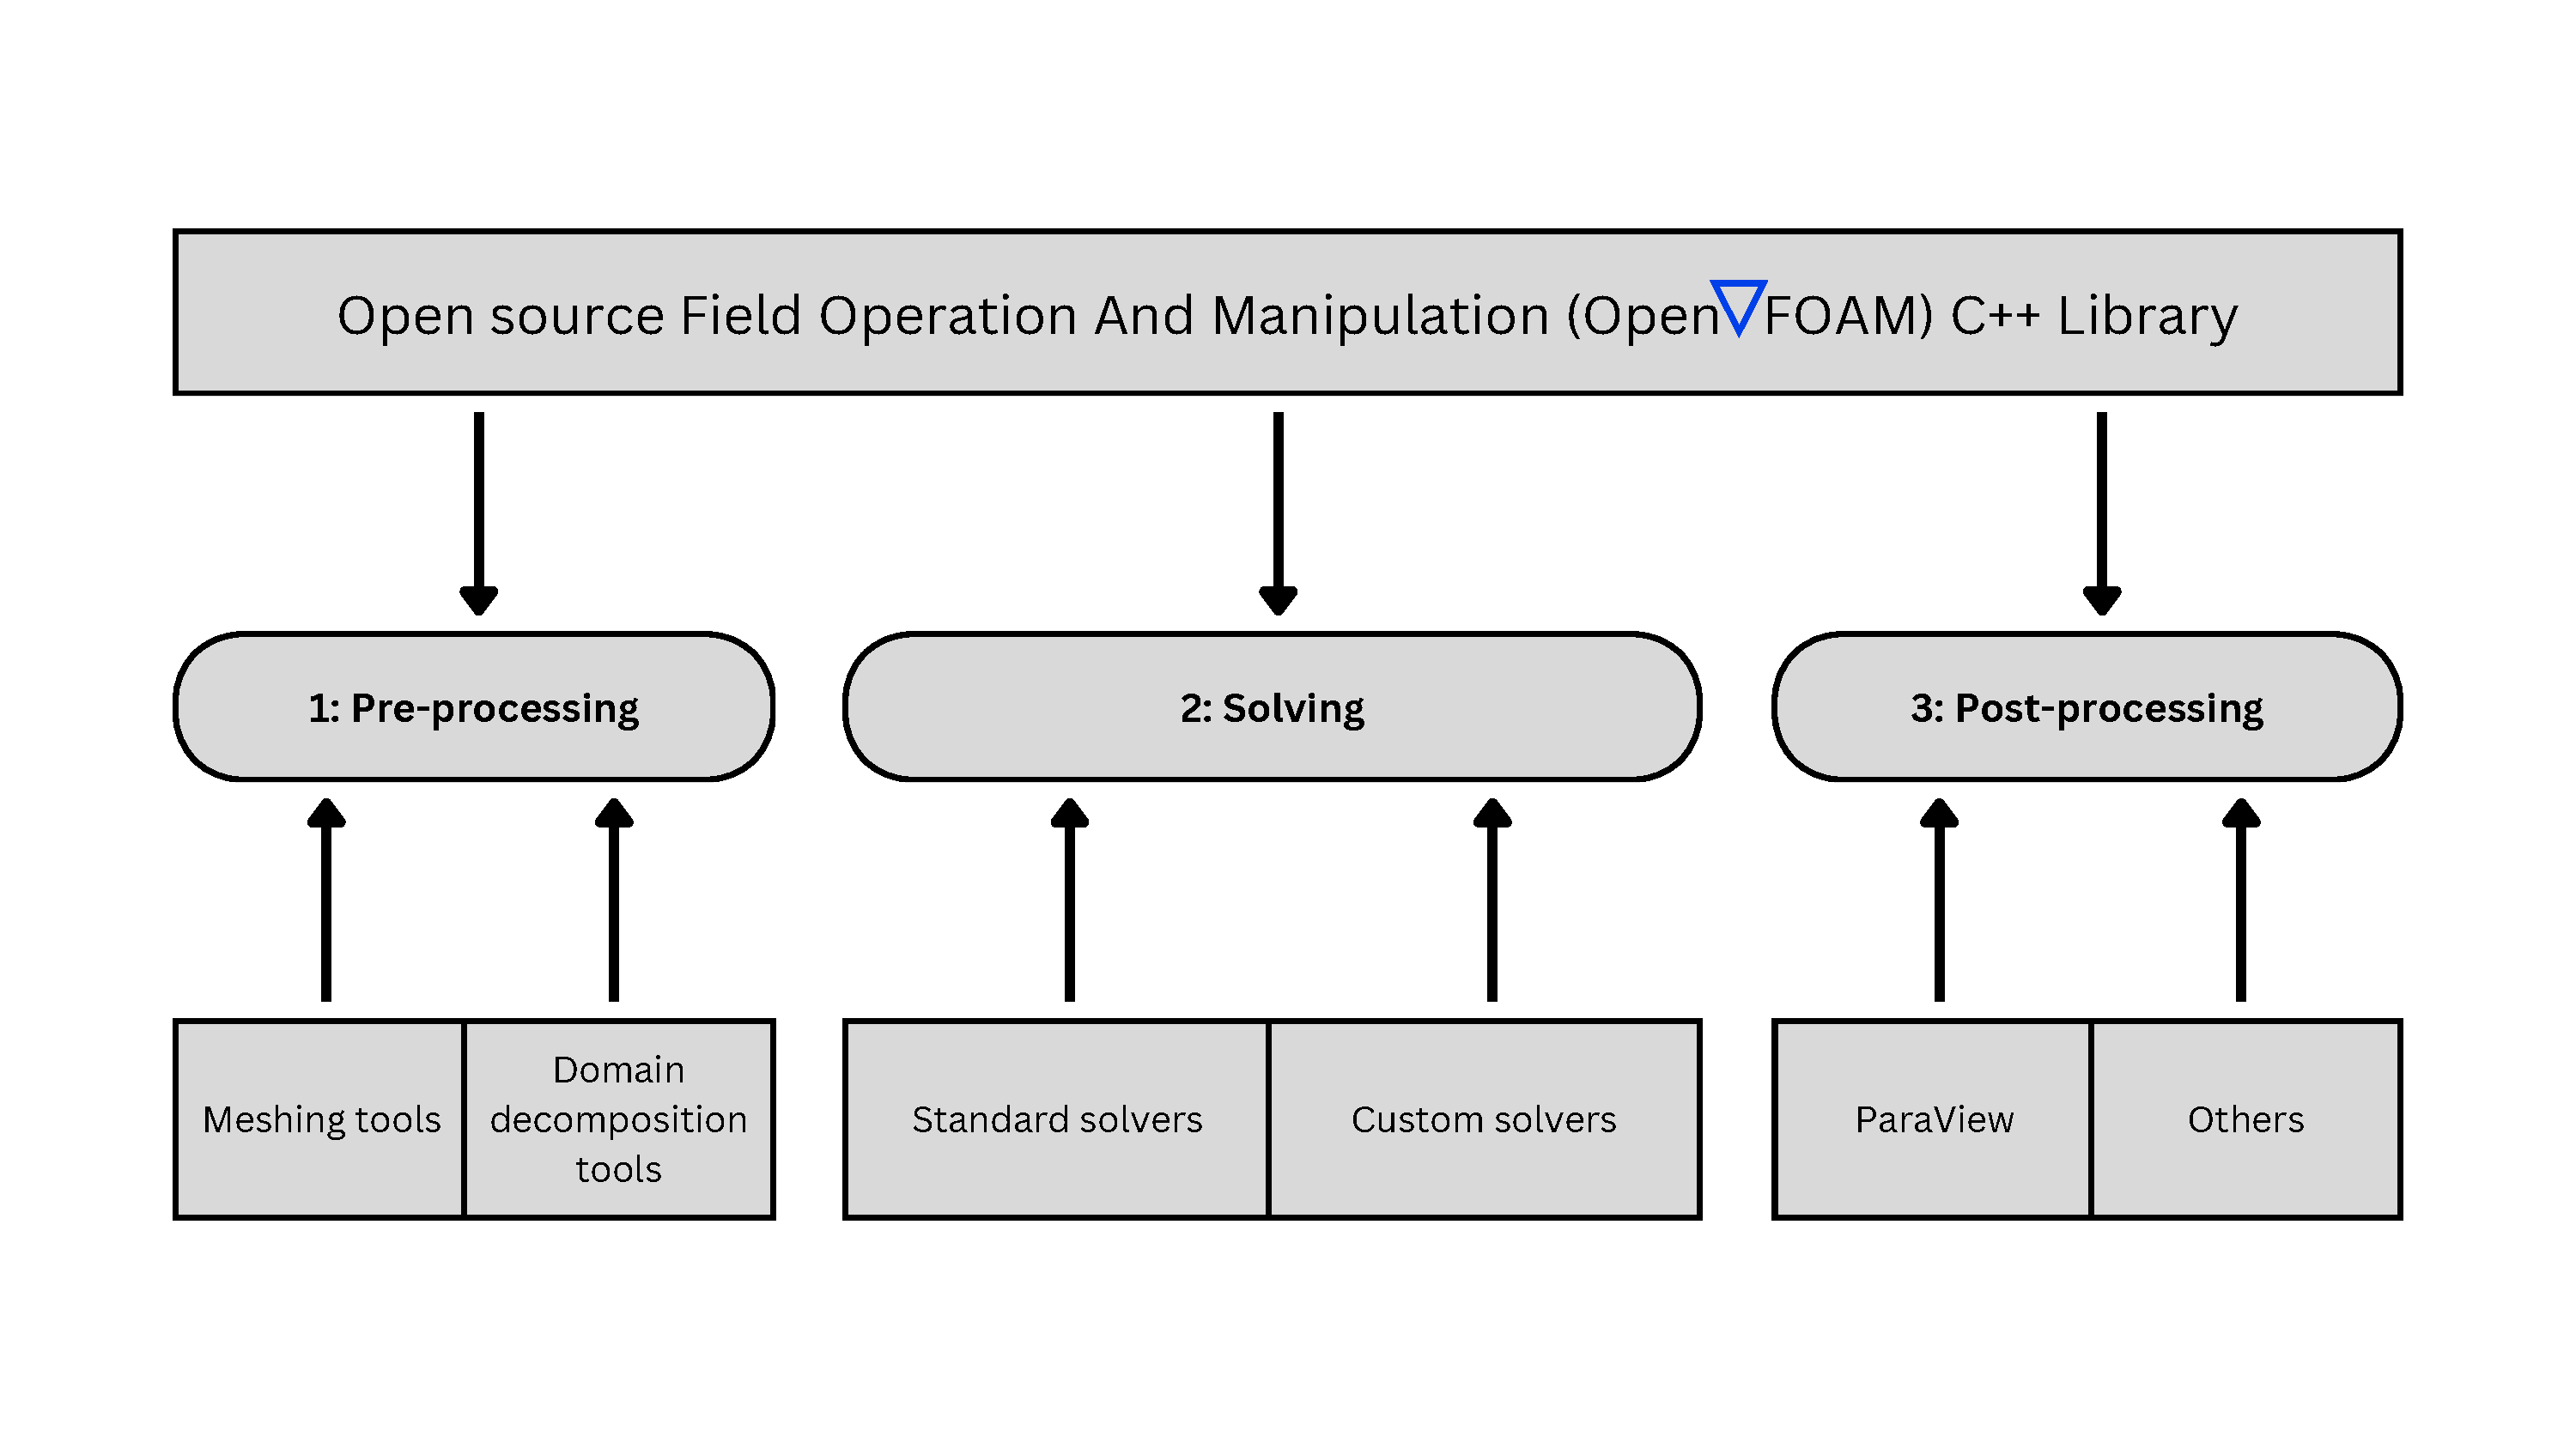
\includegraphics[width=1\linewidth]{Figures/OpenFOAM_structure}
		\caption{Overview of the OpenFOAM structure.}
		\label{OpenFOAM_structure}
	\end{figure}
	
	\noindent Figure \ref{OpenFOAM_directory_structure} shows the basic directory structure of an OpenFOAM standard case, including the essential files required to execute an application: 
	
	\begin{itemize}%[leftmargin=1]
		\item 
		\textbf{\textit{0} directory}: this is the first of the time directories required by the solver to start the simulation. In this directory, the initial condition and the boundary conditions for each physical quantity of the simulation (e.g. pressure ($p$), velocity ($U$) and temperature ($T$)) are specified.
		\item
		\textbf{\textit{constant} directory}: this folder contains the \say{polyMesh} folder where all the mesh data and the simulation boundary conditions are stored. It also contains all the properties needed to the solver, for instance the \say{thermophysicalProperties} file that specifies the thermodynamic and physical properties of the fluid or the \say{turbulenceProperties} file with the turbulence model used for the simulation.
		\item 
		\textbf{\textit{system} directory}: this folder contains the \say{controlDict} file where it is possible to define the settings of the simulation, for instance the used solver, the simulation time and the time-step. The methods for the discretization of the solved equations are specified in the \say{fvSchemes} file, while   the solvers for the discretized equations are specified in the \say{fvSolutions} file. A special mention goes to the \say{\textit{blockMesh}} utility command which creates parametric meshes with grading and curved edges. The mesh is generated from a dictionary file named blockMeshDict located in the \textit{system} directory. \say{\textit{blockMesh}} reads this dictionary, generates the mesh and writes out the mesh data files (boundary, faces, neighbour, owner and points) in the \say{polyMesh} folder, inside \say{constant}. Moreover, depending on the case problem, other files can be included in the system directory, for instance the \say{decomposeParDict} file to decompose the domain simulation into several processors such to run the simulation in parallel.
	\end{itemize}
	
	\noindent For the sake of completeness, we will describe the type of files inside the \say{polyMesh} folder. As been said above, the polyMesh subdirectory contains the followin files:
	
	\begin{itemize}
		\item \textbf{boundary}: the file boundary lists the boundaries of the domain, with the faces f each boundary type referred to as a patch and assigned a name. The type of each boundary patch (type) is declared along with its number of faces (nFaces) and the starting face (startFace),which refers to the index of the first face in the list;
		\item \textbf{faces}: the file faces represents a list of faces, with each face described by a list of indices to vertices in the points list where the first entry in the list represents face 0, the second entry represents face 1 and so on;
		\item \textbf{neighbour}: it is a list of neighbour cell labels. The number of neighbours is basically equal  the number of interior faces;
		\item \textbf{owner}: the file owner is a list in which the owner of faces are stored. The position of the owner in the list refers to the face it belongs to. The number of owners is equal to the total number of faces (interior + boundary faces);
		\item \textbf{points}: the file points is a list of vector denoting the cell vertices, with vertex 0 being the first vector in the list, vertex 1 the second vector, etc. 
	\end{itemize}
	
	\begin{figure}
		\centering
		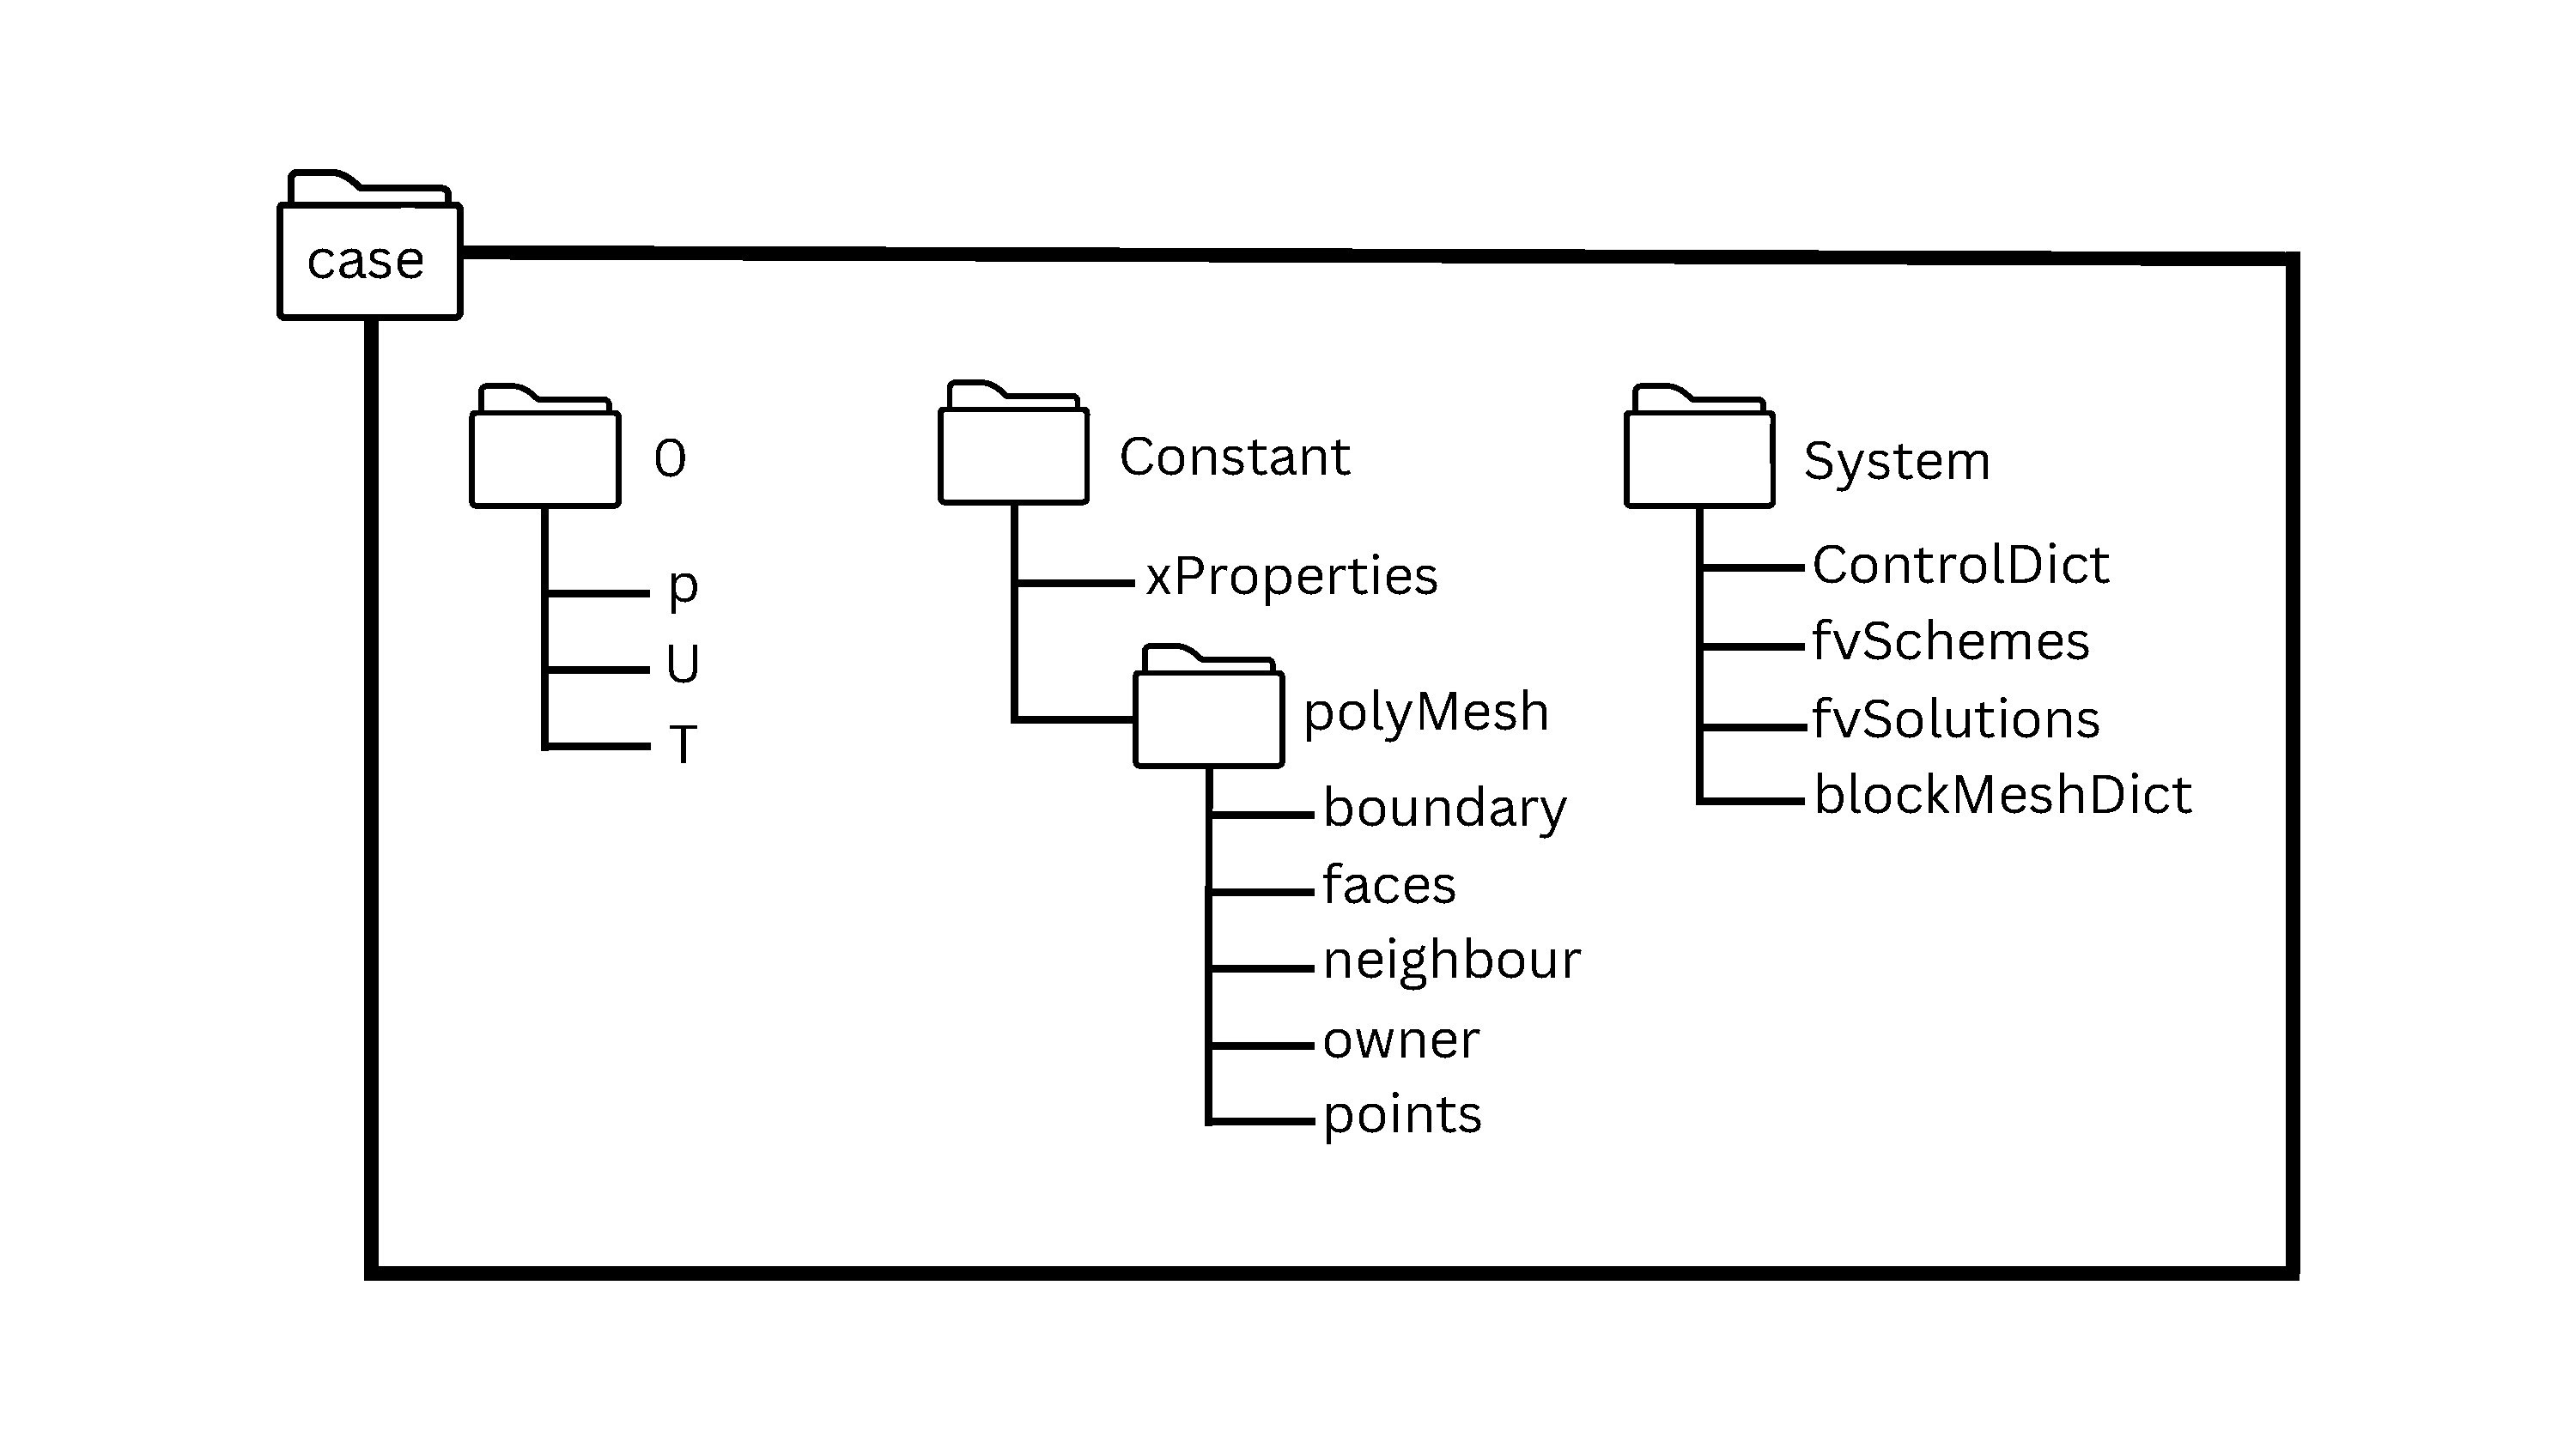
\includegraphics[origin=c, width=0.75 \linewidth]{Figures/Case_directory_structure}
		\caption{Case directory structure.}
		\label{OpenFOAM_directory_structure}
	\end{figure}
	
	\noindent OpenFOAM can handle continuum mechanics problems resolving Partial Differencial Equations (PDEs) using the Finite Volume Method over arbitrary polyhedric meshes.
	
	\newpage
	\section{The Finite Volume Method}
	
	The Finite Volume Method (FVM)\citep{ferziger2019computational} is a numerical technique that transforms the
	partial differential equations representing conservation laws over differential volumes into discrete algebraic equations over finite volumes (or elements or cells).
 	It gains popularity in CFD for being highly flexible as a discretization method. Even though it was preceded for many years by the Finite Difference (FD)\cite{crank1947practical} and Finite Element Method (FEM)\cite{clough1990original}, the FVM played a defining role in advancing the simulation of fluid flow problems and associated transport phenomena. This prominence arose from the groundbreaking work of the Computational Fluid Dynamics (CFD) group at Imperial College in the early 70s, led by Professor Spalding. Influential contributors such as \citet{gosman1969heat} and \citet{runchal1969numerical} among others, made significant strides in developing methods that shaped the field. 
	
	The FVM used in OpenFOAM follows the cell-centered logic, which is currently the most popular type of variable arrangement. This practice stores the quantities and the variables at the centroids of grid cells. More precisely, the solution domain is divided into a finite number of adjoining control volumes ($V_{p}$), and conservation equations are applied individually to each $V_{p}$. The computational node $P$ is positioned at the centroid of each control volume, where variable values are calculated. To estimate values at the surfaces of each $V_{p}$, interpolation is used to express these in terms of the nodal values located at the control volumes centers. Another way of looking at this is that FVM uses a volume integral formulation of the problem with a finite partitioning set of volumes to discretize the equations. The finite volume methods flexibility allows it to work with any type of grid, making it ideal for handling complex geometries. Additionally, the FVM ensures quantities conservation by construction, as long as the surface integrals, which represent convective and diffusive fluxes, are consistent across shared $V_{p}$ boundaries. This means that this method is inherently designed to conserve key physical quantities—such as mass, momentum, and energy—within the solution domain. This conservation property is built into the method itself, ensuring that the total amount of a conserved quantity entering or leaving a control volume (CV) equals the net accumulation or depletion of that quantity within the CV. \\
	Here we consider the general transport equation in its integral form:
	
	\begin{equation} 
		\int_{V_{p}}{{\dfrac{\partial{\rho \phi}}{\partial{t}}}}\ dV + \int_{V_{p}}{\nabla \cdot (\rho u \phi)}\ dV - \int_{V_{p}}{\nabla \cdot (\rho \Gamma_{\phi} \nabla\phi)}\ dV = \int_{V_{p}}{S_{\phi}(\phi)}\ dV
		\label{Transport equation}
	\end{equation}
	\\
	The first term of the equation \ref{Transport equation} is the integral over the volume $V_{P}$ of the temporal derivative of the product of the density $\rho$ and the generic transported quantity $\phi$, the second term is the integral of the convective term (that is the product of the density $\rho$, the velocity field $u$ and the transported quantity $\phi$), the third is the integral of the diffusion term and the last is the integral of the source term. 
	Now, let us recall the Gauss theorem which states that the outward flux of a vector field through a closed surface is equal to the volume integral of the divergence over the region inside the surface:
	
	\begin{equation}
		\int_{V}{\nabla \cdot \bar{u} \ }dV = \int_{\partial{V}}{\bar{u} \cdot \hat{n} \ dS}
		\label{Gauss theorem}
	\end{equation}
	\\
	where $\partial{V}$ is a closed surface bounding the generic control volume $V$ and $dS$ represents an infinitesimal surface element with associated normal $\hat{n}$ pointing outwards of the surface $\partial{V}$.
	
	If we use the Gauss theorem to convert the volume integrals into surface integrals, that is using equation \ref{Gauss theorem} into equation \ref{Transport equation}, we obtain the following equation
	
	\begin{equation}
		\dfrac{\partial}{\partial{t}}\int_{V_{p}}{{(\rho \phi)}}\ dV + \int_{\partial{V_{p}}}{ (\rho u \phi)\cdot \hat{n}}\ dS - \int_{V_{p}}{(\rho \Gamma_{\phi} \nabla\phi)\cdot \hat{n}}\ dS = \int_{V_{p}}{S_{\phi}(\phi)}\ dV
		\label{Transport equation_2}
	\end{equation}
	\\
	Now we can take a step further and move from the continuous domain to the discrete domain for each term.\\ 
	\indent For the convective term we have:
	
	\begin{equation}
		\int_{\partial{V_{p}}}{(\rho u \phi)} \cdot \hat{n}\ dS = \sum_{f}\int_{f}{(\rho u \phi)_{f}} \cdot \hat{n}\ dS \simeq \sum_{f} (\overline{\rho u \phi})_{f} \cdot \hat{n} \ S_{f} = \sum_{f} (\rho u \phi)_{f} \cdot \hat{n} \ S_{f}
		\label{convective discrete}
	\end{equation}
	\\
	where, in the last term, we have approximated the integrant by means of the mid point rule, which is second order accurate.
	
	For the diffusive term we have:
	
	\begin{equation}
		\begin{aligned}
			\int_{\partial{V_{p}}}{(\rho \Gamma_{\phi} \nabla \phi)} \cdot \hat{n}\ dS = \\ 
			\sum_{f}\int_{f}{(\rho \Gamma_{\phi} \nabla \phi)_{f}} \cdot \hat{n}\ dS \simeq \sum_{f} (\overline{\rho \Gamma_{\phi} \nabla \phi})_{f} \cdot \hat{n} \ S_{f} =\\
			\sum_{f} (\rho \Gamma_{\phi} \nabla \phi)_{f} \cdot \hat{n} \ S_{f}
		\label{diffusive discrete}
	\end{aligned} 
	\end{equation}
	\\
	For the source term we have:
	
	\begin{equation}
		\int_{V_{p}}{(\phi) S_{\phi}} \ dV = S_{c}V_{P} + S_{p}V_{P}\phi_{P}
		\label{source discrete}
	\end{equation}	
	\\
	This approximation is exact if $S_{\phi}$ is either constant or varies linearly with the control volume; otherwise is second order accurate. $S_{c}$ is the constant part of the source term and $S_{P}$ is the non-linear part.
	
	Using equations \ref{convective discrete}, \ref{diffusive discrete} and \ref{source discrete} into equation \ref{Transport equation_2}, we obtain the following  semi-discrete transport equation:
	
	\begin{equation}
		\dfrac{\partial}{\partial{t}}\int_{V_{p}}{{(\rho \phi)}}\ dV + \sum_{f} (\rho u \phi)_{f} \cdot \hat{n} \ S_{f} - \sum_{f} (\rho \Gamma_{\phi} \nabla \phi)_{f} \cdot \hat{n} \ S_{f} = S_{c}V_{P} + S_{p}V_{P}\phi_{P}
		\label{Discrete transport equation_2}
	\end{equation}
	\\
	where $(\rho u \phi)_{f} \cdot \hat{n} \ S_{f} = F^{C}$ is the convective flux and $(\rho \Gamma_{\phi} \nabla \phi)_{f} \cdot \hat{n} \ S_{f}=F^{D}$is the diffusive flux.
	All of this is necessary to transform the governing partial differential equations into a set of algebraic equations, one for each element in the computational domain. These algebraic equations are then assembled into a global matrix and vectors that can be expressed in the form 
	
	\begin{equation}
		A\bar{x} = \bar{b}
		\label{matrix form}
	\end{equation}
	\\
	where $A$ is the $N \times N$ coefficient matrix, $\bar{x}$ is the unknown $N$ vector variable which is defined at each interior element and at the boundary of the computational domain, and $\bar{b}$ is the vector of dimension $N$ of the known variables. One of the main advantages of the Finite Volume Method is that the techniques to solve the algebraic system of equations are independent of the discretization method, and represent the various trajectories that can be followed to obtain a solution. 
	It is important to recall that the variables are computed and stored at the centroid $P$ of the control volumes. This means that the face values in the convective and diffusive fluxes have to be computed by some form of interpolation from the centroid of the control volume at both sides of the face $f$.
	
	\newpage
	\section{Interpolation Schemes}
	
	Interpolation schemes are numerical methods used to estimate values at intermediate points within a discrete set of data or across a continuous domain. Interpolation methods range from simple approaches like linear and polynomial interpolation to more complex schemes designed to handle challenges like sharp gradients or discontinuities in data, which are common in physical simulations and engineering applications. Employing the Finite Volume Method (FVM), the partial differential equations are transformed into algebraic equations by integrating over discrete control volumes in the computational domain. This transformation requires both spatial and temporal discretization to approximate the solution within each control volume and over successive time steps.
	
	\subsection{Spatial Discretization}
	Spatial discretization is a critical component of the Finite Volume Method (FVM) when solving the Navier-Stokes equations, as it directly influences the accuracy, stability, and efficiency of the solution. In FVM, spatial discretization involves dividing the computational domain into a finite number of control volumes and approximating flow quantities and their derivatives, such as velocity and pressure, at the boundaries of these control volumes. When a the domain is two dimensional (2D) the boundaries of the control volumes is the edge of the cell and when it is three dimensional (3D) the boundary is the face of the control volume. This process enables the transformation of the continuous partial differential equations into discrete algebraic equations, which are then solved numerically.
	\\
	For high-speed flows, effective spatial discretization is essential. In such flows, sharp gradients in velocity, temperature, and pressure are common, especially near shock waves, boundary layers, and regions of rapid compression and expansion. Accurately capturing these gradients without introducing numerical errors, such as diffusion oscillations, is essential for a realistic representation of the flow field. As discussed in the review on numerical methods for high-speed flows (\citet{Pirozzoli2011}), the interpolation schemes chosen for spatial discretization play a decisive role in balancing stability and accuracy under these challenging conditions.
	\\
	In the context of the Navier-Stokes equations, spatial discretization must be applied to three terms: convective, diffusive, and gradient term. Each one requires distinct handling due to the different physical phenomena they represent. In the following paragraphs each term will be described.
	
	\subsubsection{Convective Terms}
	
	Convective terms model the transport of fluid properties, such as scalar quantities, momentum or energy, because they model the bulk motion of the flow. These terms are particularly dominant in high-speed flows, where their nonlinear nature often leads to steep gradients and discontinuities, such as shocks and expansions. Accurate resolution of these gradients is critical for capturing the essential features of compressible flows, but it poses significant numerical challenges. In fact, if the choosen discretization results inadequate, it can lead to excessive numerical diffusion with a consequent unphysical oscillations result that compromise solution fidelity.	 
	Several discretization schemes have been developed in the past decades and they are currently employed for convective terms. For instance, the \textit{Upwind Scheme}, which selects values from the upstream cell, is robust and stable, making it a popular choice for high-speed flows. However, its inherent numerical diffusion can obscure sharp gradients, making it less suitable for applications requiring high accuracy. In contrast, the \textit{Central Differencing Scheme} (CDS) achieves higher accuracy by averaging values from adjacent cells. While effective in resolving smooth gradients, CDS is prone to numerical oscillations in flows dominated by convection, limiting its applicability in scenarios involving strong discontinuities.
	\\
	To address these limitations, higher-order schemes, such as \textit{QUICK} (Quadratic Upstream Interpolation for Convective Kinematics)\cite{leonard1979stable} and \textit{MUSCL} (Monotonic Upstream-Centered Schemes for Conservation Laws)\cite{toro2013riemann}, have been developed. These methods incorporate information from multiple neighboring cells to achieve greater accuracy and reduce numerical diffusion. QUICK is particularly effective in capturing smooth gradients, while MUSCL, with its flux-limiting approach, is better suited for problems with shocks and steep gradients. Another robust and widely used  numerical scheme in CFD is the Advection Upwind Splitting Method (AUSM)\cite{LIOU_AUSM}, used for solving compressible flow problems. More precisely, it exist a rich AUSM family with  integrating enhancements that improve accuracy, stability, and efficiency, particularly in the presence of shock waves, contact discontinuities, and low-Mach-number flows. For example $AUSM^+-up$ achieves this by employing a blend of pressure-based and velocity-based flux splitting techniques while incorporating additional terms to stabilize pressure and velocity interactions. These refinements make $AUSM^+-up$ especially suitable for a broad spectrum of aerospace applications, from high-speed aerodynamics to propulsion system modeling, where precision in capturing complex flow physics is critical.
	The AUSM formulation is described herein in section \ref{AUSMsection}. The choice of the most suitable scheme in high-speed flows is a key aspect as it must balance accuracy and stability to handle the complex interplay of sharp gradients and nonlinearities. 
	\\
	The development of hybrid and adaptive schemes, which dynamically combine the strengths of multiple approaches, is an active area of research. These methods aim to achieve a balance between numerical diffusion and oscillations, making them particularly useful in simulations involving shocks, turbulence, and other complex flow features.
	
	\subsubsection{Diffusive Terms}
	Diffusion terms represent molecular diffusion processes, including viscosity and thermal conduction, which are governed by the physical properties of the fluid. Unlike convective terms, diffusion terms are generally linear, making their numerical treatment more straightforward. They are typically discretized using the \textit{Central Differencing Scheme} (CDS), which provides second-order accuracy on uniform grids. The symmetry and non-oscillatory nature of central differencing ensure stable and accurate approximation of diffusive fluxes, making it a preferred choice for the Finite Volume Method (FVM) employed in solvers such as OpenFOAM.
	\\
	Although diffusion effects are often small compared to convection in high-speed flows, their accurate representation is critical in regions where viscous effects dominate, such as boundary layers and shock-boundary layer interactions. In these areas, diffusion terms govern the transfer of momentum and energy at small scales, influencing key flow characteristics like skin friction and heat transfer. Proper discretization of these terms is essential for capturing the dynamics of shear layers, turbulence, and thermal gradients.
	\\
	Recent advances in adaptive and high-order schemes have further improved the treatment of diffusion terms, especially in simulations involving non-uniform grids or complex geometries. These methods help mitigate errors arising from grid irregularities while preserving accuracy and computational efficiency, ensuring reliable results in high-fidelity simulations.
	
	
	\subsubsection{Gradient Terms}
	
	Gradient terms, such as those arising in pressure gradient calculations, play a crucial role in fluid dynamics as they govern the acceleration and deceleration of the flow. Accurate computation of these terms is essential for capturing the dynamics of pressure-driven flows, particularly in regions with sharp pressure changes or discontinuities, such as shock waves or boundary layer separations. In computational fluid dynamics, gradient terms are typically discretized using \textit{linear central differencing}, a scheme that provides second-order accuracy on structured grids. This method is widely adopted in solvers like OpenFOAM due to its simplicity, stability, and effectiveness in regions of smooth flow.
	\\
	While \textit{linear central differencing} is effective for smooth flows, its reliance on grid uniformity can pose challenges in complex geometries or highly unstructured grids, where the accuracy of gradient calculations may deteriorate. To address these issues, advanced methods such as \textit{least squares gradient reconstruction} and \textit{weighted averaging techniques} have been developed. These approaches improve robustness and accuracy in non-uniform meshes, making them suitable for high-fidelity simulations in complex domains. 
	\\
	In high-speed flows, the accurate representation of pressure gradients is particularly critical, as errors in these terms can propagate through the solution, impacting the prediction of shock structures, expansion fans, and other key flow features. Therefore, careful selection and implementation of gradient discretization schemes are integral to achieving reliable and precise CFD results.
	
	\subsection{Flux Splitting Schemes}
	\label{AUSMsection}
	
	The story of flux splitting schemes begins in the late 1970s, when researchers were grappling with the challenge of accurately capturing shock waves and other discontinuities in compressible flow simulations. The key insight was that by splitting the flux terms into positive and negative components based on wave propagation directions, one could better handle these challenging flow features.The Godunov scheme, introduced by Sergei Godunov in 1959, represented a revolutionary approach to numerical fluid dynamics. This method solves the exact or approximate Riemann problem at cell interfaces, considering the flow as a series of interacting waves. The scheme's ability to naturally capture shock waves and maintain conservation properties made it a cornerstone of modern CFD, though its computational cost was initially seen as a drawback. Building on these foundations, the Total Variation Diminishing (TVD) scheme emerged in 1983 through the work of \citet{HARTEN1983}. TVD schemes introduced the crucial concept of limiting the numerical solution's total variation to prevent spurious oscillations near discontinuities. This advancement addressed a key limitation of earlier high-order methods which often produced unphysical oscillations near shock waves. The TVD property ensures that the numerical solution remains stable and physically meaningful, making these schemes particularly valuable for compressible flow calculations.
	One further advancement in the flux splitting domain is the development of the Advection Upwind Splitting Method (AUSM) and its subsequent iterations: AUSM+ and AUSM+-up. The AUSM (Advection Upstream Splitting Method) scheme, developed by \citet{LIOU_AUSM} in 1993, represents a more sophisticated approach to flux splitting. It cleverly separates the convective and pressure terms in the flux vector, treating them differently based on their physical nature. The scheme combines the accuracy of flux-difference splitting methods like Godunov's with the computational efficiency of flux-vector splitting approaches. What makes AUSM particularly noteworthy is its ability to accurately capture both inviscid and viscous flow features while maintaining excellent robustness and efficiency. These three schemes are interconnected through their progressive refinement of flux splitting concepts. While Godunov's scheme laid the theoretical groundwork with its wave-based approach, TVD schemes added the crucial property of solution stability, and AUSM brought everything together with a physically motivated splitting that balanced accuracy and computational efficiency. Together, they represent key milestones in the development of modern computational fluid dynamics methods.\\
	
	\noindent This section provides a comprehensive overview of these flux splitting schemes, their numerical algorithms, and their significance in addressing the challenges of all-speed flows.
	
	\subsubsection{Upwind methods}
	
	The upwinding approach, widely adopted within the gas dynamics community, is founded on the principle that the solutions of the Euler equations propagate along characteristic lines. Consequently, a stable numerical method must ensure that information is propagated in the same characteristic directions (\citet{MORETTI1979191}). Within the finite difference (FD) framework, the conventional methodology, known as flux vector splitting (\citet{STEGER1981263}), involves decomposing the flux function into positive and negative components:
	
	\begin{equation}
		f(u) = f^+(u) + f^-(u),
	\end{equation}
	\\
	where $f^+(u)$ and $f^-(u)$ correspond to non-negative and non-positive propagation velocities, respectively, i.e.,
	
	\begin{equation}
		\dfrac{df^+}{du} \geq 0 \quad \text{and} \quad \dfrac{df^-}{du} \leq 0.
	\end{equation}
	\\
	These components are discretized using left- and right-biased approximations to maintain linear stability.
	
	In the finite volume (FV) framework, upwinding is typically achieved via the flux difference splitting approach, also referred to as the Godunov method. Considering the one-dimensional (1D) scalar conservation law:
	
	\begin{equation}
		\dfrac{\partial u}{\partial t} + a(u) \dfrac{\partial u}{\partial x} = 0
		\label{conservationlaw}
	\end{equation}
	\\
	which is used as a prototype for the development of numerical methods for hyperbolic equations, we can derive its FV semi-discretization form as follows:
	
	\begin{equation}
		\dfrac{\partial \overline{u}_j}{\partial t} = \dfrac{1}{h}(f(u_{j+1/2}) - f(u_{j-1/2})),
	\end{equation}
	\\
	where $\overline{u}_j(t) = 1/h \int_{x_{j-1/2}}^{x_{j+1/2}} u(x,t) dx$ is the spacial average of the approximate solution over the cell $I_j = (x_{j-1/2},x_{j+1/2})$, a suitable reconstruction operator is used to determine approximate left and right states at the cell interfaces, $u_{j+1/2}^{\pm}$, and the interface flux $f(u_{j+1/2})$ is replaced with the numerical flux resulting from an exact (or approximate) Riemann solver, formally $\hat{f}_{j+1/2} = \textit{R}(u_{j+1/2}^{-},u_{j+1/2}^{+})$. For example, Roe's approximate Riemann solver prescribes 
	
	\begin{equation}
		\begin{aligned}
			\textit{R}(u_{j+1/2}^{-},u_{j+1/2}^{+}) = \dfrac{1}{2}(f(u_{j+1/2}^{-})+f(u_{j+1/2}^{+}))+\\
			-\dfrac{|a_{j+1/2}|}{2}(u_{j+1/2}^{+} - u_{j+1/2}^{-})
		\end{aligned}
	\end{equation}
	\\
	where $a_{j+1/2}$ is the characteristic speed associated with the intermediate state and defined as
	
	\begin{equation}
		a_{j+1/2}=(f(u_{j+1/2}^+)-f(u_{j+1/2}^-))/(u_{j+1/2}^{+}-u_{j+1/2}^{-}).
	\end{equation}
	\\
	In Godunov's original formulation, piece-wise constant reconstructions were assumed, leading to the general first-order flux
	
	\begin{equation}
		\hat{f}_{j+1/2} = \textit{R}(\overline{u}_{j},\overline{u}_{j+1})
	\end{equation}
	\\
	Upwinding has the main effect of damping the Fourier modes with the highest supported
	wave numbers, with a subsequent stabilizing effect on the numerical solution.
	
	\subsection{The AUSM Scheme}
	
	The original AUSM scheme, introduced by \citet{LIOU_AUSM} in their seminal paper \textit{“A New Flux Splitting Scheme”}, marked a significant departure from earlier flux vector and flux difference splitting methods. The key innovation of AUSM lies in its decomposition of fluxes into convective and pressure components, each treated separately to align with their respective physical characteristics.
	
	\subsubsection{Numerical Formulation}
	
	Considering the two-dimensional system of Euler equation for perfect gas:
	
	\begin{equation}
		\dfrac{\partial{U}}{\partial{t}} + \dfrac{\partial{F}}{\partial{x}} +
		\dfrac{\partial{G}}{\partial{y}} = 0
	\end{equation}
	\\
	where the velocity field is 
	
	\begin{equation}
		U =
		\begin{pmatrix}
			\rho    \\
			\rho u  \\
			\rho v  \\
			\rho E
		\end{pmatrix},
	\end{equation}
	\\
	the inviscid fluxes are 
	
	\begin{equation}
		F =
		\begin{pmatrix}
			\rho u       \\
			\rho u^2 + p \\
			\rho uv      \\
			\rho u H
		\end{pmatrix}, \
		G =
		\begin{pmatrix}
			\rho u       \\
			\rho vu		 \\
			\rho v^2 + p \\
			\rho v H
		\end{pmatrix},
	\end{equation}
	\\
	and the specific total energy is $E = e +1/2(u^2+v2) = H -p/\rho$.	
	The AUSM scheme splits the inviscid flux $F$ into two components:
	
	\begin{equation}	
		\mathbf{F} = \mathbf{F^c} + \mathbf{F^p} = 
		\begin{pmatrix}
			\rho    \\	
			\rho u  \\
			\rho v  \\
			\rho H
		\end{pmatrix} u
		+
		\begin{pmatrix}
			0 \\
			p \\
			0 \\
			0
		\end{pmatrix},
	\end{equation}
	\\
	where $F_c$ represents the convective flux, and $F_p$ represents the pressure flux. The convective terms can now be considered as passive scalar quantities convected by a suitably defined velocity $u$ at the cell interface. On the other hand, the pressure flux terms are governed by the acustic wave speeds.The two components are discretized separately and at an interface $L<\dfrac{1}{2}<R$, the convective terms can be written as function of the Mach number $M$, ensuring upwinding to handle advection accurately:
	
	\begin{equation}
		F_{1/2}^c = M_{1/2}
		\begin{pmatrix}
			\rho a 	 \\
			\rho au  \\
			\rho av  \\
			\rho aH
		\end{pmatrix}_{L/R},
	\end{equation}
	\\
	where $(M_{1/2} \simeq M_L^+ +M_R^-)$ is the value of the split Mach number at the interface (red line in figure \ref{cells}) and $a$ is the speed of sound. Various ways of defining the split Mach number exist, for instance the Van Leer\citep{van1982} splitting:
	
	\begin{equation}
		M^{\pm} = 
		\begin{cases}
			\pm\dfrac{1}{4}(M \pm 1)^2  \hspace{10 mm} if \hspace{2 mm} |M| \leq 1;\\
			\dfrac{1}{2} (M \pm |M| ),  \hspace{10 mm} if \hspace{2 mm} otherwise
		\end{cases}
	\end{equation}	
	\\
	where $M_L^+$ is the value of the left contribution of the Mach number and $M_R^-$ is the value of the right contribution of the Mach number. Also 
	
	\begin{equation}
		(\cdot)_{L/R} = 
		\begin{cases}
			(\cdot)_L  \hspace{10 mm} if \hspace{2 mm} M_L^+ \geq M_R^-\\
			(\cdot)_R  \hspace{10 mm} if \hspace{2 mm} M_L^+ < M_R^-
		\end{cases}
	\end{equation}
	\\
	where L and R are the Left and Right side of two adjacent cells respectively, as in figure \ref{cells}.
	
	\begin{figure}[t]
		\centering
		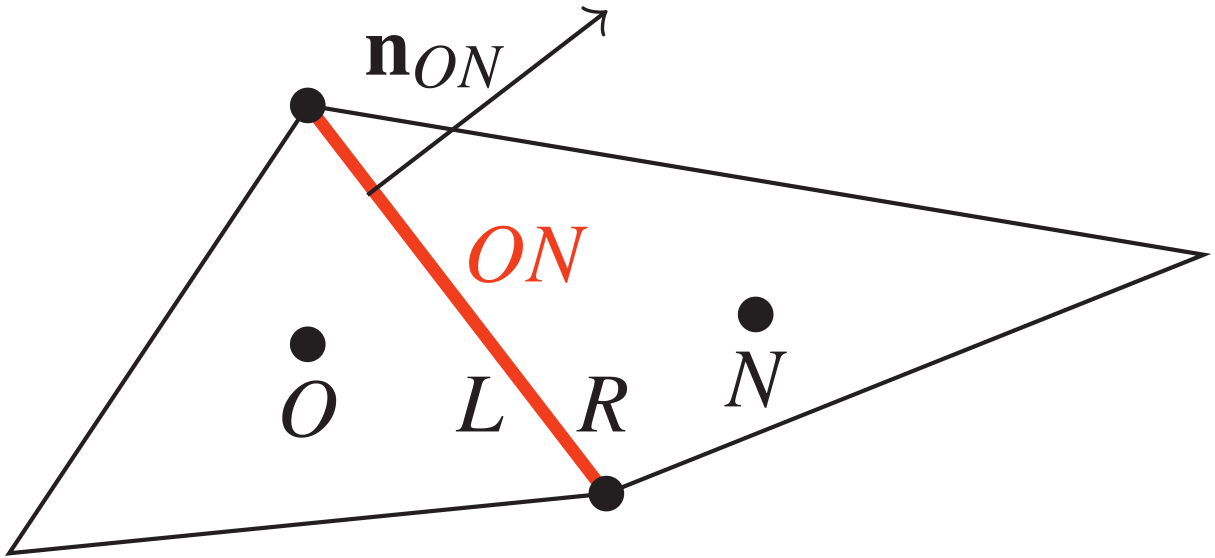
\includegraphics[width=0.4 \linewidth]{Figures/CELL.png}
		\caption{Interpolation stencil}
		\label{cells}
	\end{figure} 
	\noindent The pressure flux is treated symmetrically to ensure accurate shock resolution and smooth transitions:
	\begin{equation}
		F_p = p_{1/2} = p_L^+ + p_R^-.
	\end{equation}
	\\
	The AUSM scheme is simple and computationally efficient, providing accurate shock capturing and robust performance for subsonic and supersonic flows, sometimes with better results than the ones obtained with the Roe scheme. However, it showed limitations in maintaining stability and accuracy for low-Mach-number flows.
	
	\subsection{The AUSM+ Scheme}
	
	To address the deficiencies of AUSM, particularly removing postshock overshoot and a glitch in the slowly moving shock problem, \citet{LIOU_AUSM+} introduced the $AUSM+$ scheme in the follow-up paper. This iteration improved robustness and extended the method’s applicability to a broader range of flow conditions. In fact, the scheme is capable of exactly capturing stationary shocks and contact discontinuities, it ensures that density remains positive, which is crucial for handling strong rarefaction and near-vacuum flows, and it significantly reduces the "carbuncle" issue that affects the Roe scheme and previous AUSM implementations in blunt-body simulations.
	The AUSM+ scheme improves the splitting approach by unifying the Mach number and velocity formulations while maintaining a simple structure, making it easily adaptable to other hyperbolic systems.  
	
	\subsubsection{Algorithm}
	To implement the AUSM+ to a basic central-differencing code, it only requires the key interface quantities $(m_{j+1/2},p_{j+1/2})$ and unified numerical speed of sound $a_{j+1/2}$.  
	The Mach number is split to minimize numerical dissipation at low Mach numbers.
	
	\begin{equation}
		2m_{j+1/2} = (M_j +M_{j+1})-(\mathscr{M}_{j+1}^+ - \mathscr{M}_{j+1}^-)+(\mathscr{M}_{j}^+ - \mathscr{M}_{j}^-)-\delta m_{j+1/2},
	\end{equation}
	\\
	where
	
	\begin{equation}
		|\mathscr{M}|(M)= \mathscr{M}^+(M)-\mathscr{M}^-(M), 
	\end{equation}
	\begin{equation}
		\delta m = |\mathscr{M}|(M-{j+1})-|\mathscr{M}|(M_j) 
	\end{equation}
	\\
	and
	
	\begin{equation}
		|\mathscr{M}|(M) = 
		\begin{cases}
			|M|,					\hspace{42.5 mm} if \hspace{5 mm} |M|\geq1\\
			\dfrac{1}{2}(M^2 +1)+2\beta(M^2-1)^2, \hspace{5mm}   otherwise
		\end{cases}
	\end{equation}
	\\
	Since $|\mathscr{M}| >0 \forall M$, the absolute sign to $\mathscr{M}$ make sense. On the other hand $\Delta |\mathscr{P}|$ can be either positive or negative, depending on the sign of M:
	
	\begin{equation}
		|\mathscr{P}|(M) = 
		\begin{cases}
			sign(M),	\hspace{42.5 mm} if \hspace{5 mm} |M|\geq1\\
			\dfrac{M}{2}(3-M^2+4\alpha(M^2-1)^2), \hspace{5mm}   otherwise
		\end{cases}
	\end{equation}
	\\
	Here, the pressure flux is modified to ensure smooth transitions between subsonic and supersonic regimes. The pressure flux incorporates a blending function to adapt dynamically
	
	\begin{equation}
		2p_{j+1/2} = (p_j +p_{j+1})-\delta p_{j+1/2}
	\end{equation}
	\\
	where
	
	\begin{equation}
		\delta p_{j+1/2} = \Delta \mathscr{P}(M_{j+1})p_{j+1} - \Delta \mathscr{P} (M_{j})p_j 
	\end{equation}
	\\
	and
	
	\begin{equation}
		\Delta \mathscr{P}(M) = \mathscr{P}^+(M) - \mathscr{P}^-(M) 
	\end{equation}
	\\
	Once the quantities $(\delta p_{j+1/2},\delta m_{j+1/2})$ have been defined, the dissipative terms derived from the AUSM+ are ready to be added. Rewriting the AUSM+ flux in terms of the central-difference (CD) formula yields,
	
	\begin{equation}
		f_{j+1/2}^{AUSM^+} = f_{j+1/2}^{CD} + f_{j+1/2}^{vis} 
	\end{equation}
	\\
	where 
	\begin{equation}
		f_{j+1/2}^{vis} = f_{j+1/2}^C +f_{j+1/2}^P
	\end{equation}
	\\
	or, explicitly, the convection term is
	
	\begin{equation}
		\begin{aligned}
			f_{j+1/2}^C = - \dfrac{a_{j+1/2}}{2} \Big[\Big(\dfrac{1}{2}\delta m_{j+1/2}-|m_{j+1/2}|\Big)\Phi_j + \\
			+\Big(\dfrac{1}{2}\delta m_{j+1/2}+|m_{j+1/2}|\Big)\Phi_{j+1}\Big]
		\end{aligned}
	\end{equation}
	\\
	and the pressure term is
	
	\begin{equation}
		f_{j+1/2}^P = -\dfrac{1}{2}
		\begin{pmatrix}
			0 \\
			\delta p_{j+1/2}\\
			0
		\end{pmatrix}.
	\end{equation}
	\\
	This scheme improved stability and accuracy at low Mach numbers, enhanced shock and contact discontinuity resolution, and reduced dissipation for smooth flow regions.
	
	\subsection{The AUSM+-up Scheme}
	
	Recognizing the need for a unified framework capable of handling flows across all speeds, which could not be achieved with AUSM+, in 2006 \citet{LIOU_AUSM+-up} proposed the AUSM+-up scheme in \textit{“A Sequel to AUSM, Part II: AUSM+-up for All Speeds”}. As for its predecessors, this method integrates pressure-based and velocity-based splitting strategies, with more precise corrections that allowed the achieving of superior performances. In fact, the previous AUSM+ scheme had two critical deficiencies that affect compressible flow solvers, particularly when applied to low-speed flow predictions. These deficiencies manifest as two distinct yet interconnected problems: an intrinsic convergence instability and a fundamental inaccuracy in solution generation.
	The first issue originates at the continuum level, fundamentally tied to the governing equations' mathematical structure. This convergence challenge exists independently of the spatial discretization scheme employed, representing a deep-rooted numerical complexity. The second deficiency, however, is directly linked to the flux numerical scheme itself, offering a more tractable avenue for methodological intervention.
	Previous computational approaches, despite their practical successes, revealed significant limitations. The pressure split function exhibited a critical discontinuity at zero Mach number, necessitating arbitrary cut-off parameters that artificially constrained the method's applicability. Existing preconditioners relied on preset Mach number limitations, which fundamentally restricted the method's universal potential. The core objectives of the Liou's latest article are ambitious yet precise: to create a flux scheme that ensures convergence rates independent of Mach numbers in low-speed flows, maintains at least equivalent performance in other speed regimes, and preserves solution accuracy across the entire spectrum of flow conditions.
	
	\subsubsection{Algorithm}
	The AUSM+-up scheme introduces two critical modifications:
	
	\begin{itemize}
		\item The pressure flux incorporates an additional dissipation term proportional to the pressure difference to stabilize low-Mach-number flows.
		\item 	The convective flux is enhanced by adding a pressure-difference-driven velocity correction, ensuring robustness across all speed regimes.
	\end{itemize} 
	
	\noindent The Mach number and speed of sound at the interface are defined as:
	
	\begin{equation}
		M_{L/R} = \dfrac{u_{L/R}}{a_{1/2}},
	\end{equation}
	\\
	In the last 70 years, shock-capturing schemes have been designed starting from the features of the entropy solution of the model scalar conservation law
	\\
	where $a_{1/2}$ can be an average of $a_L$ and $a_R$. For multi-dimensional flows, $u = \mathbf{V} \cdot \mathbf{n}$, with $\mathbf{n}$ as the unit normal vector of the cell face under consideration.
	
	\noindent The following auxiliary quantities are computed:
	
	\begin{equation}
		\bar{M}^2 = \dfrac{u_L^2 + u_R^2}{2a_{1/2}^2},
	\end{equation}
	\\
	\begin{equation}
		M_o^2 = \min(1, \max(\bar{M}^2, M_1^2)),
	\end{equation}
	\\
	\begin{equation}
		f_a(M_o) = M_o (2 - M_o),
	\end{equation}
	\\
	where $f_a(M_o)$ is a scaling factor. \\
	
	\noindent Then, we can compute the mass flux and pressure fluxes as in \ref{massflux} and \ref{pressureflux}
	
	\begin{equation}
		\dot{m}_{1/2} = a_{1/2} M_{1/2} \begin{cases}
			q_L & \text{if } M_{1/2} > 0, \\
			q_R & \text{otherwise},
			\label{massflux}
		\end{cases}
	\end{equation}
	\\
	where $M_{1/2}$ is defined as:
	
	\begin{equation}
		M_{1/2} = M_+^{(4)}(M_L) + M_-^{(4)}(M_R) - \dfrac{K_p}{f_a} \max(1 - r \bar{M}^2, 0) \dfrac{p_R - p_L}{q_{1/2} a_{1/2}^2},
	\end{equation}
	\\
	with $q_{1/2} = \dfrac{q_L + q_R}{2}$.
	
	\begin{equation}
		\begin{aligned}
			p_{1/2} = P_+^{(5)}(M_L)p_L + P_-^{(5)}(M_R)p_R +\\
			- K_u P_+^{(5)}(M_L) P_-^{(5)}(M_R)(q_L + q_R) f_a a_{1/2} (u_R - u_L),
		\end{aligned}
		\label{pressureflux}
	\end{equation}
	\\
	where $P_+^{(5)}$ and $P_-^{(5)}$ are fifth-degree polynomial functions. \\
	\\
	Finally, the total flux is given by:
	
	\begin{equation}
		F_{1/2} = \dot{m}_{1/2} \tilde{w}_{L/R} + p_{1/2},
	\end{equation}
	\\
	where $\tilde{w}_{L/R}$ represents the convected variables, selected upwinded based on the sign of $\dot{m}_{1/2}$. \\
	
	\noindent With these modifications, the AUSM+-up scheme achieves some advantages:
	\begin{itemize}
		\item Unified handling of incompressible, subsonic, transonic, and supersonic flows.
		\item Improved accuracy for steady and unsteady low-Mach-number flows.
		\item Robust shock and contact discontinuity resolution.
	\end{itemize}
	
	\noindent Finally we can say that the AUSM family has profoundly impacted CFD, providing reliable tools for simulating a wide range of aerodynamic and thermodynamic problems. Applications span from aerospace engineering to turbomachinery, internal combustion engines, and atmospheric modeling. The AUSM+-up scheme, in particular, has become a standard choice for many high-fidelity solvers, owing to its ability to handle diverse flow phenomena without compromising stability or accuracy.
	
	\newpage
	\subsection{Shock Capturing Schemes}
	The shock-capturing method applies a uniform discretization scheme across all points and achieves stabilization by incorporating numerical dissipation, which prevents the emergence of Gibbs oscillations. In contrast, the shock-fitting method treats shock waves as true discontinuities, governed by their own algebraic equations and it employs the Rankine-Hugoniot relations as nonlinear boundary conditions to connect the states on either side of the discontinuity.
		
	\subsubsection{Classical methods}
	
	In the late 1950s, shock-capturing schemes have been designed starting from the features of the entropy solution of the model scalar conservation law \ref{conservationlaw}, as follows:
	
	\begin{itemize}
		\item $\mathbf{Monotonicity \ preservation}$ which states that initially monotone data remain monotone for all times;
		\item $\mathbf{Total \ Variation \ Diminishing}$ (TVD) which in mathematical form states
		\begin{equation}
			TV(u(\cdot,t_2))\leq TV(u(\cdot,t_1)), \quad \forall t_2 \geq t_1
		\end{equation}
		\\
		where $TV(u(\cdot,t))$ denotes the total variation of $u$, as follows for a discrete sequence $u_j$
		\begin{equation}
			TV(u) = \sum_{j=1}^{n} |u_{j+1}-u_j|
		\end{equation}
		\item $\mathbf{Monotonicity}$: we consider two solutions of equation \ref{conservationlaw}, for instance $u(x,t)$, $v(x,t)$.\\ The monotonicity property states that if $u(x,0)\leq v(x,0) \quad \forall (x)$ then 
		\begin{equation}
			u(x,t)\leq v(x,t) \quad \forall (x,t)
		\end{equation}
	\end{itemize}
	
	\noindent Owing to the availability of rigorous theorems ensuring the convergence of TVD schemes to weak solutions and monotone schemes to entropy solutions, many shock-capturing implementations satisfying these conditions have appeared in the literature. Even though TVD schemes gained wide success in the 1980s, the main problem of monotone schemes is that they can achieve at best first-order accuracy with a conseguent loss of accuracy at both smooth and non-smooth extrema. This led researchers to pursue alternatives for constructing uniformly high-order accurate shock-capturing schemes. 
	The Essentially NonOscillatory (ENO) schemes introduced by  \citet{HARTEN1983} address this issue by computing the numerical flux via a high-order reconstruction over an adaptively chosen stencil that minimizes interpolation across discontinuities, thus reducing Gibbs oscillations. ENO reconstructions of order $r$ ensure that the increase in total variation is limited to $O(h^r)$, which keeps the total variation uniformly bounded. However, the free adaptation of stencils in ENO schemes can cause convergence problems and loss of accuracy. Building on these ideas, Weighted Essentially NonOscillatory (WENO) schemes were later introduced by \citet{LIU1994}. These schemes construct a single high-order numerical flux as a convex linear combination of several lower-order polynomial reconstructions over a set of staggered stencils. The weights of the stencils are chosen so that maximum formal accuracy is achieved in smooth regions while almost zero weight is given to reconstructions that cross a discontinuity. Subsequent research has focused on enhancing the performance of WENO schemes, especially by improving their behavior in smooth regions. 
	
	\subsubsection{Hybrid Methods}
	This class of methods enhances a basic spectral-like scheme with shock-capturing capabilities by either locally switching to a conventional shock-capturing method or by selectively incorporating the dissipative component of a shock-capturing method acting as a nonlinear filter. A key role in this class of schemes is played by shock sensors that must be defined in such a way that numerical dissipation is effectively confined in shocked regions, so that it does not pollute smooth parts of the flow field. For instance, to analyze the interaction between an isotropic turbulent field and a planar shock wave, we could use a hybrid discretization of a high-order compact scheme and a high-order shock-capturing ENO scheme but, in this case, the shock location is approximately known, so the switch between the two schemes can be decided a priori. \citet{ADAMS1996} initially explored a truly adaptive hybrid discretization, combining a baseline compact upwind scheme with a fifth-order ENO scheme. A simple switching mechanism, based on the local gradients of the flux vector components, was employed to identify critical cells. These cells were then surrounded by buffer cells on each side to preclude oscillations caused by the coupling of different properties schemes. In 2002, \citet{PIROZZOLI2002} extended the approach by formulating a fully conservative scheme that blends a fifth-order compact upwind numerical flux with a seventh-order WENO flux, employing a switching mechanism determined by the local density gradient. Even though hybrid schemes are a valid alternative to the classical methods above, it appears that sometimes the coupling between two methods may give rise to an unstable system, thus requiring a deeper investigation. However, if the two schemes used in the coupling are both dissipative, then the coupled system is strongly stable, therefore endorsing the use of upwind shock-capturing schemes around discontinuities. 
	The Jameson–Schmidt–Turkel (JST\cite{JST1981}) scheme, introduced in 1981, employs central differencing for spatial discretization and incorporates artificial dissipation terms to maintain numerical stability and accurately capture shock waves. The JST scheme computes numerical fluxes using a central difference method with added artificial dissipation to ensure stability and prevent oscillations in shock-dominated flows. These components are controlled by sensors based on pressure variations. The scheme has also been reformulated as a total-variation-diminishing (TVD) scheme, aligning it with modern high-resolution methods.    
	Suppose that the scalar conservation law is the one in equation \ref{conservationlaw} which can be approximated by the semidiscrete scheme
	
	\begin{equation}
		\Delta x \dfrac{d v_j}{d t} + \hat{f}_{(j+1/2)} -  \hat{f}_{(j-1/2)} = 0
		\label{semidiscretescheme}
	\end{equation} 
	\\
	where $v_j$ represents the average value of $u$ in cell $j$, and $f_{(j+1/2)}$ is the numerical flux across the interface separating cells $j$ and $j+1$. 
	Introducing artificial diffusion, the JST numerical flux can be defined as follows:
	
	\begin{equation}
		\hat{f}_{(j+1/2)} = \hat{f}^C_{(j+1/2)} - d_{(j+1/2)}
	\end{equation}
	\\
	where the diffusive flux has the following form
	
	\begin{equation}
		\begin{aligned}
			d_{(j+1/2)} = \epsilon^2_{(j+1/2)} \Delta v_{(j+1/2)} +\\
			- \epsilon^4_{(j+1/2)}(\Delta v_{(j+3/2)} - 2\Delta v_{(j+1/2)} + \Delta v_{(j-1/2)})
		\end{aligned}		
	\end{equation}
	\\
	with $\Delta v_{(j+1/2)} = v_{j+1} -v_j$, which becomes:
	
	\begin{equation}
		d_{(j+1/2)} = \epsilon^2_{(j+1/2)} (v_{j+1}-v_j) - \epsilon^4_{(j+1/2)}(v_{j+2}-3v_{j+1}+3v_j-v_{j-1})
	\end{equation}
	\\
	Here, we can see that the dissipation term consists of a second-order component (to handle small oscillations) and a fourth-order component (to reduce excessive dissipation in smooth regions). 
	Let $a_{(j+1/2)}$ be the numerically estimated wave speed
	
	\begin{equation}
		a_{j+1/2} = 
		\begin{cases}
			\dfrac{f_{j+1}-f_j}{v_{j+1}-v_j}, \quad v_{j+1} \neq v_j \\[0.6cm]
			\dfrac{\partial f}{\partial u}\bigg\rvert_{u=v_j}, \quad v_{j+1} = v_j 
		\end{cases}.
	\end{equation}
	\\
	So the JST scheme is TVD whenever $v_j$ and $v_{j+1}$ is an extremum,
	
	\begin{equation}
		\epsilon^2_{(j+1/2)} \geq \dfrac{1}{2}|a_{(j+1/2)}|, \quad \epsilon^4_{(j+1/2)} = 0.
	\end{equation}
	\\
	To construct coefficients $\epsilon^2_{(j+1/2)}$ and $\epsilon^4_{(j+1/2)}$ that satisfy the previous conditions, it is necessary to define the following function:
	\begin{equation}
		R(u,v) = \bigg|\dfrac{u-v}{|u|+|v|} \bigg|^q
	\end{equation}
	\\
	where $q\geq1$. Then, if $u$ and $v$ have opposite signs, 
	\begin{equation}
		R(u,v) = 1.
	\end{equation}
	\\
	Now, set
	\begin{equation}
		\begin{cases}
			\epsilon^2_{(j+1/2)} = \alpha_{(j+1/2)}Q_{j+1/2} \\[1mm]
			\epsilon^4_{(j+1/2)} = \beta_{(j+1/2)}(1-Q_{j+1/2})
		\end{cases}
	\end{equation} 
	\\
	where 
	\begin{equation}
		Q_{j+1/2} = R(\Delta v_{(j+3/2)}, \Delta v_{(j-1/2)}).
	\end{equation}
	\\
	Because $\Delta v_{(j+3/2)}$ and $\Delta v_{(j-1/2)}$ have opposite signs if either $v_j$ or $v_{j+1}$ is an extremum, the scheme will be a local extremum diminishing (LED) scheme if
	\begin{equation}
		\alpha_{(j+1/2)} \geq \dfrac{1}{2}|a_{(j+1/2)}|.
	\end{equation}
	\\
	Typically, 
	\begin{equation}
		\beta_{(j+1/2)} = \textit{k}_4|a_{(j+1/2)}|
	\end{equation}
	\\
	where in the case of steady-state calculations, $\textit{k}_4$ can be tuned to maximize the rate of convergence to a steady state.
	This realization of the JST scheme is actually an example of a symmetric TVD scheme.
	Overall, the formulation of the JST scheme was guided by a number of design principles such as: 
	
	\begin{itemize}
		\item The scheme should be in conservation form to ensure
		satisfaction of the shock jump conditions, according to the theorem of \citet{LAXWENDROFF}.
		\item There should be second-order accuracy in smooth regions of
		the flow.
		\item Shock waves should be captured without overshoots or
		oscillations, at least in the steady state (but overshoots during the
		transient phase would be tolerated).
		\item The steady state should be independent of the time evolution.
		\item The scheme should be stable when using variable local time steps
		at a fixed CFL number to accelerate convergence to a steady state.
		\item The discrete steady-state solution should have constant
		stagnation enthalpy, consistent with properties of the true steady-state
		solutions. 
	\end{itemize}
	
	\noindent Moreover, the artificial flux of the Jameson-Schmidt-Turkel (JST) scheme in equation \ref{Jamesonsensor} was also used by \citet{DUCROS1999} to modify the original nonlinear filtering approach, initially introduced by \citet{YEE1999199} who designed one of the first low-dissipative, shock-capturing algorithm. In fact, Ducros replaced the Harten \cite{HARTEN1983} switch, which is designed to be almost unity near shocks and almost zero in smooth parts of the flow, with the product of the Jameson sensor and another shock sensor, that is known as the "Ducros Sensor".
	
	\begin{equation}
		\psi_{j}= \dfrac{|v_{j+1}-2v_{j}+v_{j-1}|}{|v_{j+1}+2v_{j}+v_{j-1}|}, \quad 0 \leq \psi_{j} \leq 1.
		\label{Jamesonsensor}
	\end{equation}
	
	\paragraph{Ducros Sensor} 
	The Ducros sensor, introduced by \citet{DUCROS1999}, is a tool designed to distinguish between compressible shocks and other flow features such as vortices, thus aiding in the adaptive application of numerical dissipation. It is defined as:
	
	\begin{equation}
		\phi = \dfrac{(\nabla \cdot \mathbf{u})^2}{(\nabla \cdot \mathbf{u})^2 + (\nabla \times \mathbf{u})^2 + \epsilon},
	\end{equation}
	\\
	where ($\nabla \cdot \mathbf{u}$) is the flow divergence, ($\nabla \times \mathbf{u}$) is the vorticity magnitude, and $\epsilon$ is a small positive constant to prevent division by zero. The sensor takes values between 0 and 1, with values close to 1 indicating regions dominated by compression (shocks), and values close to 0 identifying vortex-dominated regions. This makes it particularly effective for hybrid and nonlinear filtering schemes, where dissipation needs to be selectively introduced. Extensions of the Ducros sensor have been employed in direct numerical simulations and large-eddy simulations, as it can reduce the risk of incorrectly identifying vortices as shocks, ensuring a better distinction of flow dynamics. This enhances computational efficiency and accuracy in solving compressible turbulent flows with shocks. 
	Later studies conducted by \citet{garnier2001class} showed that the Ducros sensor is capable of distinguishing turbulent
	fluctuations from shocks better than the Harten \cite{HARTEN1983} switch.
	
	\newpage
	\subsection{Temporal Discretization}
	
	Temporal discretization allows the solution to evolve over time, which is an essential process in unsteady simulations. In computational fluid dynamics, the choice of time discretization scheme plays a significant role in determining both accuracy and computational efficiency of the solution. In the following paragraphs, the main time discretization methods are described, analysing for each their stability, accuracy and computational cost properties.
	
	\subsubsection{Explicit Time Discretization}
	
	Explicit schemes are numerical methods in which the solution at the next time step is calculated directly from the known values at the current time step. A commonly used explicit method is the \textit{forward Euler}\cite{darwish2016finite} scheme, which approximates the time derivative as:
	
	\begin{equation}
	 F(\phi^n) \approx \dfrac{\phi^{n+1} - \phi^n}{\Delta t}.
	\label{forwardEuler}
	\end{equation}
	\\
	Here, $\phi^{n+1}$ represents the unknown solution at the next time step, $\phi^n$ is the known solution at the current time step and $\Delta t$ is the time step size.
	So the unknown flux $\phi^{n+1}$ can be evaluated starting from equation \ref{forwardEuler} as follows:
	
	\begin{equation}
		\phi^{n+1} \approx \ \phi^n + F(\phi^n) \ \Delta t.
		\label{forwardEuler1}
	\end{equation}
	\\
	Starting from a fixed $\Delta t$ and knowing the function $F(\phi^n$, the stored quantities of the known values at the current time $\phi^n$ can be used to evaluate the unknown values of the quantities at the next time $\phi^{n+1}$. This makes explicit schemes straightforward to implement and computationally efficient.
	Explicit schemes are conditionally stable and require the time step size $\Delta t$ to satisfy specific stability criteria, such as the Courant-Friedrichs-Lewy (CFL) condition. For example, in advection-dominated problems, the CFL condition imposes the following constraint:
	
	\begin{equation}
	\Delta t \ \leq \ C_{max} \ \dfrac{\Delta x}{|\mathbf{u}|},
	\label{CFL}
	\end{equation}
	\\
	where $\Delta x$ is the spatial grid resolution and $|\mathbf{u}|$ is the characteristic velocity of the flow. Failure to meet this criterion may result in numerical instability. The value of $C_{max}$ changes with the method used to solve the discretised equation, especially depending on whether the method is explicit or implicit. If an explicit solver is used then typically $C_{max} \leq 1$. Implicit solvers are usually less sensitive to numerical instability, so $C_{max} > 1$. 
    The accuracy of explicit schemes depends on their formulation.
	In general, in order for this kind of schemes to be accurate the CFL require a very low $\Delta t$ (e.g. for a dimensionless time, that would correspond to an order of magnitude of $10^{-6}$). This requires large computation times to be sure the simulation has come to convergence.
	The \textit{forward Euler} method is first-order accurate, meaning that its error decreases linearly with the time step size. Higher-order explicit schemes, such as \textit{Runge-Kutta} methods, provide improved accuracy by incorporating additional intermediate steps within each time step.
	Explicit schemes have a low computational cost per time step compared to other schemes because they avoid solving coupled systems of equations. Instead, each time step involves simple arithmetic operations, which makes these methods suitable for problems where computational efficiency is a priority.
	Explicit schemes are particularly suitable for problems where the solution evolves rapidly, and small time steps are naturally required for accuracy. They are commonly employed in transient simulations dominated by advection or in problems involving wave propagation, where the small time scales ensure stability and precision.
	
	\subsubsection{Implicit Time Discretization}
	
	Implicit schemes are widely employed in CFD, particularly for simulations where numerical stability is a primary concern, such as in unsteady flow problems with large time steps or in systems involving strong coupling between physical processes.
	This kind of schemes provide a robust approach for solving time-dependent problems by incorporating unknown future states into the formulation. This characteristic allows implicit methods to operate with larger time steps compared to explicit schemes, making them particularly advantageous for stiff problems commonly encountered in computational fluid dynamics. A widely used implicit time discretization is the \textit{Backward Euler}\cite{darwish2016finite} method, which approximates the time derivative as:
	
	\begin{equation}
		F(\phi^{n+1}) \approx \dfrac{\phi^{n+1} - \phi^n}{\Delta t},
	\end{equation}
	\\
	where $\phi^{n+1}$ is the unknown variable at the new time step, $\phi^n$ is the known value at the current time step, and $\Delta t$ is the time step size.
	
	This scheme is said to be implicit because the calculation of the unknown variable at the next time step $\phi^{n+1}$ is implicitly depending on itself:
	
	\begin{equation}
		\phi^{n+1} \approx \ \phi^n + F(\phi^{n+1}) \ \Delta t.
	\label{backwardEuler1}
	\end{equation}
	\\
	It is now well known that the accuracy of implicit schemes depends on their formulation. The backward Euler method is first-order accurate and unconditionally stable for many linear problems. For scenarios demanding improved accuracy, the \textit{Crank-Nicolson}\citep{crank1947practical} method - a second-order implicit scheme - can be employed. This method averages the time derivative between the current and next time steps, providing greater accuracy but sometimes introducing oscillations in highly nonlinear systems or when large time steps are used. 
	Implicit schemes are unconditionally stable for many linear problems, allowing the use of larger time step sizes without the risk of numerical instability. This is particularly beneficial for stiff systems, such as high Reynolds number flows or strongly coupled multi-physics problems.
	Implicit schemes are also computationally expensive as they require solving a coupled system of algebraic equations at each time step. This cost can become significant for large-scale problems in which the use of efficient solvers and preconditioners to ensure feasibility are required.
	Despite their computational cost, their unconditional stability and ability to handle stiff equations make them a very powerful and are commonly used in many CFD software programs.
	
	\newpage
	\section*{Application in OpenFOAM}
	In OpenFOAM, the selection of interpolation schemes for spatial and temporal terms is specified in the \texttt{fvSchemes} and \texttt{fvSolution} configuration files. The \texttt{fvSchemes} file determines the spatial interpolation schemes for divergence, gradient, and Laplacian terms, while \texttt{fvSolution} configures the temporal schemes and solvers for each variable. For high-speed flows, the selection of schemes is particularly critical, as these flows are sensitive to both numerical diffusion and oscillations. Typically, an initial solution might employ an upwind scheme for stability, which can then be refined with higher-order schemes, such as \textit{Roe}\cite{ROE1981357}, \textit{TVD}\cite{HARTEN1983} or \textit{AUSM}\cite{LIOU_AUSM}, for improved accuracy. The Roe scheme is a popular approximate Riemann solver that linearizes the flux Jacobian to achieve high accuracy and ensure proper wave propagation by capturing discontinuities with minimal numerical dissipation. The Godunov scheme, on the other hand, is a fundamental first-order method that employs the exact solution of the Riemann problem to determine fluxes at cell interfaces, ensuring robust shock capturing, albeit with relatively high dissipation. To overcome the excessive numerical diffusion of first-order methods, Total Variation Diminishing (TVD) schemes were introduced, incorporating non-oscillatory high-order reconstructions such as MUSCL (Monotonic Upstream-Centered Schemes for Conservation Laws) to enhance solution accuracy while maintaining stability. The Advection Upstream Splitting Method (AUSM) family of schemes takes a different approach by splitting convective and pressure fluxes, offering superior accuracy in capturing compressible flow features like shocks and contact discontinuities, especially in transonic and supersonic regimes. Together, these methods highlight the evolution of upwind techniques, balancing accuracy, stability, and computational efficiency for complex flow problems.
	
	\section{OpenFOAM solvers}
		
	OpenFOAM is known for its flexibility and extensive range of solvers tailored to specific simulation needs. The solvers in OpenFOAM are broadly categorized into incompressible and compressible solvers, addressing fluid flow scenarios depending on the fluid’s compressibility and the physical phenomena being modeled. Incompressible solvers are designed for flows where density variations are negligible, such as low-speed air or water flows. Examples include simpleFoam for steady-state turbulent flows, pimpleFoam for transient simulations using the SIMPLE and PIMPLE algorithms, and icoFoam for laminar, transient flows. On the other hand, compressible solvers handle flows where changes in density due to pressure and temperature variations are significant, as in high-speed aerodynamics, supersonic flows and combustion processes. Examples include rhoSimpleFoam and rhoPimpleFoam for steady and transient compressible flows, respectively, and rhoCentralFoam, which leverages a central difference scheme for shock-dominated flows. Beyond these categories, OpenFOAM also includes specialized solvers for heat transfer, multiphase flows, chemical reactions, and electromagnetics. For instance, solvers like chtMultiRegionFoam enable conjugate heat transfer analysis, while interFoam and twoPhaseEulerFoam address multiphase flow problems. Each solver is tailored to specific applications, allowing users to simulate a wide range of industrial and research problems with high accuracy and computational efficiency. Furthermore, the modularity of OpenFOAM enables customization of solvers, providing unparalleled flexibility to engineers and researchers.
	
	\subsection*{Simple, Piso and Pimple Methods}
	
	Developed in the early 1970s by Professor Brian Spalding and his student Suhas Patankar \cite{patankar1980numerical} at Imperial College London, the SIMPLE algorithm has become a cornerstone in CFD research and applications. Over the years, it has been widely adopted and extensively applied by researchers to address a broad range of fluid flow and heat transfer problems, solidifying its position as a key method in the numerical simulation of fluid dynamics.
	The SIMPLE (Semi-Implicit Method for Pressure-Linked Equations) algorithm is widely used in OpenFOAM for addressing the pressure-velocity coupling inherent in the Navier-Stokes equations. This coupling arises from the incompressibility condition, which requires that the velocity field remain divergence-free.
	\\
	The SIMPLE algorithm is primarily designed for steady-state simulations: in fact it do not contain any time derivation in the equations. In this approach, the momentum equation is first solved using an initial guess for the pressure field to obtain an intermediate velocity field. Since this velocity field does not necessarily satisfy the continuity equation, a pressure correction equation is derived from the continuity condition. This correction is applied iteratively to adjust the pressure field and subsequently the velocity field until the solution converges. The SIMPLE algorithm is computationally efficient for steady-state problems due to its iterative nature, but it can converge slowly for problems with strong nonlinearities or transient effects.
	\\
	On the other hand, the PISO (Pressure Implicit with Splitting of Operators) algorithm\cite{ISSA198666} is also a  method for solving the implicity discretised, time-dependent, Navier-Stokes equations, but it uses a non-iterative approach within each time step, which makes it computationally efficient for transient problems and it is better suited for unsteady simulations. As for the SIMPLE algorithm, the PISO algorithm begins with a solution of the momentum equation using an initial guess for the pressure field, leading to an intermediate velocity field. A pressure correction equation is then derived to ensure that the velocity field satisfies the continuity equation. After the pressure field is corrected, the velocity field is updated accordingly. Unlike SIMPLE, PISO may include additional corrector steps within a single time step to improve the accuracy of the solution. These corrector steps are optional and are determined by the specific requirements of the problem.
	\\
	The primary difference between SIMPLE and PISO lies in their application and strategy. SIMPLE is iterative across all equations and is optimized for steady-state problems, where convergence to a final solution is required. On the other hand, PISO avoids iteration across time steps and is designed for transient problems, allowing larger time steps while maintaining numerical stability. Both methods are implemented in OpenFOAM with configurable parameters in the \texttt{fvSolution} dictionary, allowing users to adapt the algorithms to specific cases.
	\\
	Lastly, the PIMPLE algorithm, is a hybrid scheme obtained from SIMPLE and PISO: it combines the iterative robustness of SIMPLE with the transient capabilities of PISO, making it versatile for both steady-state and transient problems. Within each time step, PIMPLE employs an outer iteration loop akin to SIMPLE, predicting the velocity field and applying pressure corrections until a specified convergence criterion is met. Simultaneously, it integrates the inner correction steps characteristic of PISO to achieve tighter pressure-velocity coupling. This dual-level approach allows PIMPLE to handle large time steps and complex flow conditions with improved stability, making it particularly effective for simulations involving turbulence or multiphase flows.
	
	\subsection*{simpleFoam}
	\texttt{simpleFoam} is a steady-state, pressure-based solver for incompressible flows, using the SIMPLE algorithm. It is commonly used in industrial and aerodynamic applications where steady-state conditions are dominant.
	
	\subsection*{pimpleFoam}
	\texttt{pimpleFoam} is a transient, pressure-based solver for incompressible flows, using the PIMPLE algorithm. It is robust for large time steps and high Courant number simulations.
	
	\subsection*{pisoFoam}
	\texttt{pisoFoam} is a transient, pressure-based solver for incompressible flows, using the PISO algorithm. It is widely used for unsteady turbulent flow simulations.
	
	\subsection*{rhoSimpleFoam}
	\texttt{rhoSimpleFoam} is a steady-state, pressure-based solver for compressible flows. It employs the SIMPLE  algorithm, making it suitable for steady aerodynamics and heat transfer applications.
	
	\subsection*{rhoPimpleFoam}
	\texttt{rhoPimpleFoam} is a transient, pressure-based solver for compressible flows. It uses the PIMPLE algorithm, providing stability for high Courant number simulations.
		
	\subsection*{rhoPisoFoam}
	\texttt{rhoPisoFoam} is a transient, pressure-based solver for compressible flows, using the PISO algorithm. It is suitable for low and moderate Mach number flows where transient behavior is important.
		
		
	\subsection*{rhoCentralFoam}
	
	\texttt{rhoCentralFoam} is a transient, density-based solver designed for compressible flows. It employs a central-upwind scheme suitable for high-speed flows, including transonic, supersonic, and hypersonic regimes. The solver effectively captures shock waves and discontinuities using a robust numerical method based on the Kurganov and Tadmor central scheme.
	\\
	\texttt{rhoCentralFoam} employs a central-upwind scheme with the following features:
	\begin{itemize}
		\item Kurganov-Tadmor central scheme for shock capturing.
		\item Flux splitting into left-going and right-going components.
		\item MUSCL (Monotonic Upstream-Centered Scheme) for second-order spatial accuracy.
		\item Runge-Kutta time integration.
		\item Harten-Lax-van Leer (HLL)-type numerical flux formulation.
	\end{itemize}
	These features enhance stability and accuracy in capturing shocks, rarefactions, and contact discontinuities effectively. While it has some limitations, particularly for steady-state problems, it remains a robust, efficient, and widely used solver in the computational fluid dynamics (CFD) community.
		
	\subsection*{sonicFoam}
	\texttt{sonicFoam} is a transient, pressure-based solver for compressible flows that supports subsonic, transonic, and supersonic conditions. It uses the PISO algorithm for time marching and pressure-velocity coupling.\\
	\\	
	The following table presents a comparative summary of the solvers described above, highlighting the flow regime, numerical approach, and their capability to handle shocks and turbulence.	
	\begin{table}[h]
		\centering
		\resizebox{\textwidth}{!}{
		\begin{tabular}{|c|c|c|c|c|}
			\hline
			Solver & Flow Regime & Approach & Shock Handling & Turbulence Support \\
			\hline
			\texttt{simpleFoam} & Incompressible, steady-state & Pressure-based & Low & RANS \\
			\texttt{pimpleFoam} & Incompressible, transient & Pressure-based & Low & RANS, LES \\
			\texttt{pisoFoam} & Incompressible, transient & Pressure-based & Low & RANS, LES \\
			\texttt{rhoSimpleFoam} & Compressible, steady-state & Pressure-based & Moderate & RANS \\
			\texttt{rhoPimpleFoam} & Compressible, transient & Pressure-based & Moderate & RANS, LES \\
			\texttt{rhoPisoFoam} & Compressible, transient & Pressure-based & Moderate & RANS, LES \\
			\texttt{rhoCentralFoam} & Compressible, high-speed & Density-based & Good & RANS, LES \\
			\texttt{sonicFoam} & Compressible, subsonic/supersonic & Pressure-based & Moderate & RANS, LES \\
			\hline
		\end{tabular}}
		\caption{Comparison of OpenFOAM Solvers for incompressible and compressible flows}
		\label{tab:comparison}
	\end{table}
	

	
	\newpage
	\section{CFD Methodologies}
	
\	\subsection{Reynolds-Averaged Navier-Stokes (RANS)}
	The RANS approach is one of the most common methods used in turbulence modeling. It implies averaging the Navier-Stokes equations over time, which effectively smooths out fluctuations in turbulence to provide a steady-state solution. This method greatly simplifies computational requirements and is particularly useful for applications where the flow is stable or slightly unsteady. RANS models are widely used in industrial applications because of their robustness and low computational costs. However, they may be less accurate in predicting complex flows with significant separation or strong instability.
	The key to obtain RANS equations is to use the Reynolds decomposition which divide the velocity field into a mean component ($U$) and a fluctuating component ($u'$):
	
	\begin{equation}
		u = U  + u'
	\end{equation}
	\\	
	The Reynolds-averaged Navier Stokes (RANS) equation in tensor form, derived from the incompressible form of the Navier Stokes equations, can be written as:
	
	\begin{equation}
		\frac{\partial (\rho U_i)}{\partial t} + \frac{\partial (\rho U_i U_j)}{\partial x_j} = -\frac{\partial P}{\partial x_i} + \frac{\partial}{\partial x_j} \left[ \mu \left( \frac{\partial U_i}{\partial x_j} + \frac{\partial U_j}{\partial x_i} \right) - \rho \overline{u_i' u_j'} \right]
		\label{RANS}
	\end{equation}
	\\
	where $\mu$ is the molecular viscosity.	The Reynolds decomposition introduces a term called Reynolds stress ($-\rho \overline{u'_i u'_j}$) when applied to the Navier-Stokes equations, that can be modeled with the Boussinesq hypothesis \cite{boussinesq1877essai} as follows:
	
	\begin{equation}
		- \rho \overline{u_i' u_j'} = \mu_t \left( \frac{\partial U_i}{\partial x_j} + \frac{\partial U_j}{\partial x_i} - \frac{2}{3} \frac{\partial U_k}{\partial x_k} \delta_{ij} \right) - \frac{2}{3} \rho k \delta_{ij}
	\end{equation}
	\\
	where $\mu_t$ is the turbulent eddy viscosity and $\delta_{ij}$ is the Kronecker Delta:
	\begin{equation}
		\delta_{ij} = 
		\begin{cases}
			1, if i=j \\
			0, if i\neq j
		\end{cases}
	\end{equation}
	\\
	The primary problem with RANS equations is that there are more unknowns than equations. The system of equations for the first moments depends on correlations involving pairs of variables (second moments) and RANS equations developed for these pair correlations involve triple correlations. For example, the conservation equation for the Reynolds stress correlation, $\overline{u_i' u_j'}$:
	\begin{equation}
		\begin{aligned}
			\frac{\partial u_i u_j}{\partial t} + U_k \frac{\partial u_i u_j}{\partial x_k} + \frac{\partial u_i u_j u_k}{\partial x_k} = - u_i u_k \frac{\partial U_j}{\partial x_k} - u_j u_k \frac{\partial U_i}{\partial x_k} + \\
			-\frac{1}{\rho} \left( u_i \frac{\partial p}{\partial x_j} + u_j \frac{\partial p}{\partial x_i} \right)  
			- 2 \nu \frac{\partial u_i}{\partial x_k} \frac{\partial u_j}{\partial x_k} + \nu \frac{\partial^2 u_i u_j}{\partial x_k^2} + \\
			+ g \alpha \left( u_j T' \delta_{i3} + u_i T' \delta_{j3} \right)
		\end{aligned}
	\end{equation}
	\\
	and triple correlations appear in the third term on the left. Similar conservation equations for the triple correlations involve quadruple correlations, and the equations for the quadruple correlations depend on fifth-order correlations, and so on. This problem persists at all correlation levels and is known as the closure problem in turbulence. At the present time there are three approaches to the closure problem. The first, known as RANS closure
	modeling, involves terminating the equation hierarchy at a given level and closing the resulting system of equations with models developed from dimensional analysis, 	intuition, symmetry requirements, and experimental results. The second, known as direct numerical simulations (DNS) involves numerically solving the time-dependent equations of motion and
	then Reynolds averaging the computational output to determine mean-flow quantities. The third, known as large-eddy simulation (LES), combines elements of the other two and involves some modeling and some numerical simulation of large-scale turbulent fluctuations.
	
	\subsection{RANS closure models}
	The closure problem arising from Reynolds-averaging of the equations of fluid motion has lead to the development of approximate models to close systems of RANS equations. Because
	of the practical importance of such models for weather forecasting and performance prediction for engineered devices, RANS-closure modeling efforts have existed for more than a century and continue to this day. This section presents a truncated overview of the essential elements leading to the most known turbulence models that can be divided into two categories: the one equation models like the Spalart-Allmaras model, and the two-equation models like the $k-\varepsilon$ model and the $k-\omega$ model.
	
	\subsubsection{Spalart-Allmaras model}
	The Spalart-Allmaras (SA) model is a one-equation turbulence model\cite{SPALARTALLMARAS} designed primarily for aerodynamic flows, particularly those involving wall-bounded and external flows around airfoils, wings, and vehicles. This model introduces a transport equation for a modified \textbf{eddy viscosity} ($\tilde{\nu}$), making it computationally efficient while still capturing important turbulence effects. \\
	The turbulent \textbf{eddy viscosity} is given by:
	
	\begin{equation}
		\nu_t = \tilde{\nu} f_{v1}, \quad f_{v1} = \frac{\chi^3}{\chi^3 + C_{v1}^3}, \quad \chi := \frac{\tilde{\nu}}{\nu}
	\end{equation}
	\\
	and the transport equation for the modified eddy viscosity is:
	
	\begin{equation}
		\begin{aligned}
			\frac{\partial \tilde{\nu}}{\partial t} + u_j \frac{\partial \tilde{\nu}}{\partial x_j} = C_{b1} [1 - f_{t2}] \tilde{S} \tilde{\nu} 
			+ \frac{1}{\sigma} \left\{ \nabla \cdot [( \nu + \tilde{\nu}) \nabla \tilde{\nu}] + C_{b2} | \nabla \tilde{\nu} |^2 \right\} +\\
			- \left[ C_{w1} f_w - \frac{C_{b1}}{\kappa^2} f_{t2} \right] \left( \frac{\tilde{\nu}}{d} \right)^2 + f_{t1} \Delta U^2
		\end{aligned}
	\end{equation}

	where:
	
	\begin{equation}
		\tilde{S} \equiv S + \frac{\tilde{\nu}}{\kappa^2 d^2} f_{v2}, \quad f_{v2} = 1 - \frac{\chi}{1 + \chi f_{v1}}
	\end{equation}
	
	\begin{equation}
		f_w = g \left[ \frac{1 + C_{w6}^6}{g^6 + C_{w6}^6} \right]^{1/6}, \quad g = r + C_{w2} (r^6 - r), \quad r \equiv \frac{\tilde{\nu}}{\tilde{S} \kappa^2 d^2}
	\end{equation}
	
	\begin{equation}
		f_{t1} = C_{t1} g_t \exp \left( -C_{t2} \frac{\omega_t^2}{\Delta U^2} [d^2 + g_t^2 d_t^2] \right)
	\end{equation}
	
	\begin{equation}
		f_{t2} = C_{t3} \exp(-C_{t4} \chi^2)
	\end{equation}
	
	\begin{equation}
		S = \sqrt{2 \Omega_{ij} \Omega_{ij}}
	\end{equation}
	\\
	The rotation tensor is given by
	\begin{equation}
		\Omega_{ij} = \frac{1}{2} \left ( \frac{\partial{u_i}}{\partial{x_j}} - \frac{\partial{u_j}}{\partial{x_i}}\right ),
	\end{equation}
	\\
	$d$ is the distance from the closest surface and $\Delta{U^2}$ is the norm of the difference between the velocity at the trip (usually zero) and that at the field point we are considering. 
	All the constant are written in table \ref{table:SAconstants}:
	
	\begin{table}[h]
		\centering
		\renewcommand{\arraystretch}{1.2} % Adjust row height
		\begin{tabular}{c c}
			\hline
			\textbf{Constant} & \textbf{Value} \\ 
			\hline
			$\sigma$  & $2/3$ \\
			$C_{b1}$  & $0.1355$ \\
			$C_{b2}$  & $0.622$ \\
			$\kappa$  & $0.41$ \\
			$C_{w1}$  & $\frac{C_{b1}}{\kappa^2} + \frac{(1 + C_{b2})}{\sigma}$ \\
			$C_{w2}$  & $0.3$ \\
			$C_{w3}$  & $2$ \\
			$C_{v1}$  & $7.1$ \\
			$C_{t1}$  & $1$ \\
			$C_{t2}$  & $2$ \\
			$C_{t3}$  & $1.1$ \\
			$C_{t4}$  & $2$ \\
			\hline
		\end{tabular}
		\caption{Spalart-Allmaras constants}
		\label{table:SAconstants}
	\end{table}
	
	\noindent There are several approaches to adapting the model for compressible flows. In all cases, the turbulent dynamic viscosity is computed from
	
	\begin{equation}
		\mu_t = \rho \tilde{\nu} f_{v1}
	\end{equation}
	\\
	where $\rho$ is the local density.
	
	
	\subsubsection{$k-\varepsilon$ model}
	This model solves transport equations for turbulent kinetic energy (k) and dissipation rate ($\varepsilon$):
	
	\begin{equation}
		\frac{\partial \rho k}{\partial t} + \frac{\partial \rho k u_i}{\partial x_i} = \frac{\partial}{\partial x_j}\left[\left(\mu +\frac{\mu_t}{\sigma_k}\right)\frac{\partial k}{\partial x_j}\right] + P_k + P_b - \rho \varepsilon - Y_M + S_k
	\end{equation}
	\\	
	\begin{equation}
		\frac{\partial \rho \varepsilon}{\partial t} + \frac{\partial \rho \varepsilon u_i}{\partial x_i} = \frac{\partial}{\partial x_j}\left[\left(\mu+ \frac{\mu_t}{\sigma_\varepsilon}\right)\frac{\partial \varepsilon}{\partial x_j}\right] + C_{1 \varepsilon}\frac{\varepsilon}{k} (P_k +C_{3\varepsilon} P_b) - C_{2 \varepsilon}\rho \frac{\varepsilon^2}{k} + S_{\varepsilon
		}
	\end{equation}
	\\
	Where $u_i$ represents the component of the velocity in the corresponding direction, $E_{ij}$ represents the component of the strain tensor, $\mu_t$ represents the turbulent viscosity and has the following equation:
	
	\begin{equation}
		\mu_t = \rho C_{\mu} \frac{k^2}{\varepsilon}
	\end{equation}
	\\
	The equation contains some calibration constants $\sigma_k$, $\sigma_{\varepsilon}$, $C_{1\varepsilon}$ and $C_{2\varepsilon}$. The value of these constants are derived from experimental results, and the standard values used are:
	$C_{\mu }=0.09$, $\sigma_k = 1.00$, $\sigma_{\varepsilon} = 1.30$, $C_{1\varepsilon} = 1.44$ and $C_{2\varepsilon} = 1.92$.
	
	\subsubsection{$k-\omega$ model}
	The $k-\omega$ turbulence model is widely used for simulating turbulent flow conditions within the framework of Reynolds-averaged Navier-Stokes (RANS) models. It falls under the category of two-equation models, which augment the conservation equations with two additional transport equations (PDEs). These equations account for the temporal and spatial variations of turbulent energy ($k$) and specific turbulent dissipation rate ($\omega$). $k$ represents the turbulent kinetic energy, indicating the energy content of turbulence, while $\omega$ characterizes the rate at which turbulence dissipates per unit of $k$. This dissipation rate is also known as the turbulence scale.
	The transport equation for turbulent kinetic energy  and for the turbulent dissipation rate are given in equation \ref{tke_equation} and \ref{specific_dissipation_rate_equation} as described in \citet{Wlicox_k-omega_model} paper:
	
	\begin{equation}
		\frac{\partial (\rho k)}{\partial t} + \frac{\partial}{\partial x_j} (\rho u_j k) =
		\rho \tau_{ij} \frac{\partial u_i}{\partial x_j} - \rho \varepsilon + \frac{\partial}{\partial x_j} \left[ \left( \mu + \sigma^* \frac{\rho k}{\omega} \right) \frac{\partial k}{\partial x_j} \right]
		\label{tke_equation}
	\end{equation}
	\\	
	\begin{equation}
		\begin{aligned}
			\frac{\partial (\rho \omega)}{\partial t} + \frac{\partial}{\partial x_j} (\rho u_j \omega) =
			\alpha \frac{\omega}{k} \rho \tau_{ij} \frac{\partial u_i}{\partial x_j} - 	\beta \rho \omega^2 
			+ \sigma_d \frac{\rho}{\omega} \frac{\partial k}{\partial x_j} 	\frac{\partial \omega}{\partial x_j} +
			\\
			+ \frac{\partial}{\partial x_j} \left[ \left( \mu + \sigma \frac{\rho 	k}{\omega} \right) \frac{\partial \omega}{\partial x_j} \right]
		\end{aligned}
		\label{specific_dissipation_rate_equation}
	\end{equation}
	\\
	where $u_i$ represents the component of the velocity in the corresponding direction, $\tau_{ij}$ is the shear stress tensor, $\mu$ is the dynamic viscosity, $\nu_t = k/\omega$ is the kinematic eddy viscosity, $\varepsilon =\beta^* \omega k$, $\alpha = 0.52$, $\beta^* = 0.09$ and $\sigma^*=0.60$, $\sigma = 0.50$ and 
	
	\begin{equation}
		\sigma_d =
		\begin{cases}
			0, \hspace{13.5mm} \frac{\partial k}{\partial x_j} 	\frac{\partial \omega}{\partial x_j} \leq 0 \\
			\sigma_{d0}, \hspace{10mm} \frac{\partial k}{\partial x_j} 	\frac{\partial \omega}{\partial x_j} > 0
		\end{cases},
		\hspace{8mm}\sigma_{d0} =0.125
	\end{equation}	
	\\
	Specifically, the model is as accurate for attached boundary layers, backward-facing steps, and mildly separated incompressible flows. Also, $k-\omega$ model predicts  reasonably close agreement with measured properties of shock-separated flows for transonic, supersonic, and hypersonic regimes.
	
	\subsection{Unsteady RANS (URANS)}
	URANS extends the RANS approach by allowing time-dependent variations in the flow field, making it capable of capturing unsteady phenomena. It still uses Reynolds averaging of the Navier-Stokes equations but does not calculate the time-averaged flow as rigorously as RANS. This means that URANS can model large-scale transient flow characteristics and oscillatory behaviors that are typical in many practical engineering systems, such as vortex detachment from building corners. Although URANS improves RANS in terms of capturing instability, it still uses eddy viscosity models that may not adequately resolve finer turbulent structures. Additionally, while URANS requires more computational resources than RANS, it remains significantly more efficient than higher-fidelity turbulence models like Large Eddy Simulation (LES) or Delayed Detached Eddy Simulation (DDES). This balance between accuracy and efficiency makes URANS a practical choice for many engineering applications where large-scale unsteady behavior plays a critical role. However, URANS has limitations, particularly in handling complex turbulent flows. Due to its reliance on eddy-viscosity models, it may struggle to accurately predict fine turbulent structures. Moreover, despite being time-dependent, URANS still averages the flow over time, potentially smoothing out important transient details. Another drawback is its reduced effectiveness in strongly separated flows, as it lacks the refinement of LES or hybrid methods in capturing separation and reattachment phenomena. Despite these limitations, URANS remains a widely used approach in engineering applications requiring a compromise between accuracy and computational efficiency.

	\subsection{Large Eddy Simulation (LES)}
 	Large Eddy Simulation (LES) is a mathematical model used in CFD to  study turbulent phenomena. Initially proposed in 1963 by Joseph \citet{smagorinsky1963general} for modeling atmospheric currents, it is still the subject of great interest both because of its possible developments and because it stands as a middle ground between RANS-type modeling (faster but more approximate) and DNS direct numerical simulation (more exact but computationally very expensive). LES basic idea is to reduce computational cost by ignoring the smallest length scales, which are the most expensive to resolve, through low-pass filtering of the Navier–Stokes equations. This filtering can be seen as a combination of time- and spatial-averaging, effectively removing small-scale information from the numerical solution. However, this information is not irrelevant, as its influence on the flow field must still be modeled.
	The governing equations of LES are obtained by filtering the Navier-Stokes equations both for incompressible flows and compressible flows. 
	The former approach generate the filtered advection term that can be split up, following 
	
	\begin{equation}
		\overline{u_i u_j} = \tau_{ij} + \bar{u}_i\bar{u}_j
	\end{equation}
	\\
	where $\tau_{ij}$ is the residual stress tensor, so that the filtered incompressible momentum balance equation becomes: 
	\begin{equation}
				\frac{\partial{\bar{u_i}}}{\partial{t}} + \frac{\partial}{\partial{x_j}} (\bar{u_i}\bar{u_j}) = -\frac{1}{\rho}\frac{\partial{\bar{p}}}{\partial{x_i}} + 2\nu \frac{\partial{\bar{S_{ij}}}}{\partial{x_j}} -\frac{\partial{\tau_{ij}}}{\partial{x_j}}
	\end{equation}
	\\
	where $\bar{S}_{ij}$ is the filtered strain rate tensor:
	
	\begin{equation}
		\bar{S}_{ij} = \frac{1}{2}\left(\frac{\partial \bar{u}_i}{\partial x_j} + \frac{\partial \bar{u}_j}{\partial x_i}\right)
	\end{equation}
	\\
	The Smagorinsky model treats dissipation of kinetic energy at sub-grid scales as analogous to molecular diffusion and so, it relates the filtered strain rate tensor to the stress tensor:
	
	\begin{equation}
		\tau_{ij} - \frac{1}{3}\delta_{ij}\tau_{kk} = -2 \nu_t \bar{S}_{ij}
	\end{equation}
	\\
	where $nut_t$ is the the turbulent eddy viscosity 
	\begin{equation}
		\nu_t = (C_s\Delta)^2|\bar{S}|\bar{S}_{ij}
	\end{equation}
	
	\subsection{Detached Eddy Simulation (DES)}
	DES combines RANS and LES approaches, with the transition controlled by:
	
	\begin{equation}
		\tilde{d} = \min(d, C_{DES}\Delta)
	\end{equation}
	
	where $d$ is the wall distance and $C_{DES}$ is a model constant.
	
	\subsection{Direct Numerical Simulation (DNS)}
	DNS resolves all scales down to the Kolmogorov scales:
	
	\begin{equation}
		\eta = \left(\frac{\nu^3}{\varepsilon}\right)^{1/4} \quad \text{(length scale)}
	\end{equation}
	
	\begin{equation}
		\tau_\eta = \left(\frac{\nu}{\varepsilon}\right)^{1/2} \quad \text{(time scale)}
	\end{equation}
	
	\subsection{Grid Resolution Requirements}
	\begin{itemize}
		\item RANS: $y^+ \approx 30$ for wall functions or $y^+ < 1$ for low-Reynolds number models
		\item LES: $\Delta x^+ \approx 50\text{--}150$, $\Delta y^+ < 1$, $\Delta z^+ \approx 15\text{--}40$
		\item DNS: $\Delta x^+ \approx 10$, $\Delta y^+ < 1$, $\Delta z^+ \approx 5$
	\end{itemize}
	
	\subsection{Computational Cost}
	The computational requirements for DNS scale with Reynolds number as:
	
	\begin{equation}
		N \sim Re^3
	\end{equation}
	
	where $N$ is the total number of grid points required.
	
	\chapter{Methodology}
	\label{chap:methodology}
    This solver addresses the numerical challenges of simulating fluid dynamics in situations involving significant temperature variations, density changes, and complex energy transfer mechanisms. By employing advanced numerical discretization techniques and solving coupled energy and momentum conservation equations, rhoEnergyFoam provides researchers and engineers with a powerful computational framework for investigating thermodynamic phenomena across diverse applications, from aeronautical engineering to industrial thermal management systems. The following methodology section will delve into the mathematical formulation, numerical algorithms, and computational strategies that underpin the rhoEnergyFoam solver, elucidating the precise numerical methods used to transform fundamental conservation laws into computationally tractable algorithms capable of accurately predicting fluid behavior under complex thermodynamic conditions.
	
	\section{rhoEnergyFoam}
	RhoEnergyFoam is a high-fidelity numerical solver for solving Navier-Stokes equations in the compressible field. The solver exploits the predictive capabilities of low-diffusion numerical schemes useful for the applied study of flows around complex geometries. The spatial discretization of convective terms in the Navier-Stokes equations is based on a robust energy-preserving numerical flow, and the numerical diffusion inherited from the AUSM scheme is added limitedly to the vicinity of shock waves, or wherever spurious numerical oscillations are detected. The solver is capable of preserving the total kinetic energy in the nonviscous limit, and bears significantly less numerical diffusion than typical industrial solvers, with greater predictive power, as demonstrated through a series of test cases including DNS \citep{Modesti_2018}, LES \citep{LARSSON201615-00418} and URANS of turbulent flows \citep{SPALART2000252}.
	
	Let's consider the Navier-Stokes equations for a compressible ideal gas, integrated over an arbitrary volume $V$
	
	\begin{equation}
		\dfrac{d}{dt}\int_V \textbf{u} \ dV + \sum_{i=1}^{3} \int_{\partial{V}} (\textbf{f}_i-\textbf{f}_i^{\nu}) \cdot n_i \ dS = 0
	\end{equation}
	
	The simulation of turbulent compressible flows remains a cornerstone in computational fluid dynamics (CFD), requiring high-fidelity solvers capable of capturing complex flow behaviors in industrial and academic settings. This work introduces an advanced numerical solver for the compressible Navier-Stokes equations, prioritizing low numerical diffusion and enhanced energy conservation. The core of this solver lies in its use of an energy-preserving flux computation combined with the Advection Upstream Splitting Method (AUSM) for shock regions. This novel integration seeks to address the inherent limitations of many industrial CFD solvers, which rely on first or second-order discretization methods stabilized through upwind schemes and implicit segregated algorithms. These traditional methods often exhibit excessive numerical diffusion, which compromises their ability to resolve fine-scale turbulent structures, especially in scenarios such as large-eddy simulations (LES) or direct numerical simulations (DNS). By contrast, the solver described in this study incorporates features common in academic approaches, such as high-order discretization and explicit time integration, to achieve a balance between computational efficiency and predictive accuracy.
	
	The mathematical foundation of the solver begins with the discretization of the compressible Navier-Stokes equations. The governing equations, integrated over an arbitrary control volume, are expressed in terms of conservative variables, convective fluxes, and viscous fluxes. The numerical fluxes are split into convective and pressure components, with the central part evaluated to preserve kinetic energy. This formulation ensures discrete conservation of total kinetic energy in the inviscid limit, a property essential for accurate turbulence modeling. The central flux, however, is insufficient for practical applications involving shocks or unstructured meshes. To address this, the solver employs a localized addition of numerical diffusion derived from the AUSM scheme. This diffusion is activated dynamically based on a shock sensor that evaluates local smoothness, ensuring minimal dissipation in smooth regions while effectively capturing shocks. The shock sensor uses velocity and length scales to detect zones requiring additional numerical stabilization, maintaining stability without compromising accuracy.
	
	Implementation within OpenFOAM, a widely used open-source CFD framework, underscores the solver's practicality. OpenFOAM’s flexibility allows for seamless integration of the proposed numerical techniques, including the use of its existing primitives for spatial discretization and boundary condition handling. The solver supports three operational modes tailored to different flow regimes: Mode A for fully resolved smooth flows (e.g., DNS), Mode B for unresolved smooth flows (e.g., DES or RANS), and Mode C for shocked flows. This modularity enables users to adjust the solver’s behavior based on the specific demands of their simulations, optimizing computational resources while maintaining accuracy.
	
	The solver's capabilities are validated through a comprehensive set of test cases, beginning with canonical flows such as decaying isotropic turbulence and the Taylor-Green vortex. In the isotropic turbulence test, the solver’s energy-preserving properties are evident, with Mode A ensuring exact conservation of kinetic energy over multiple eddy turnover times. This contrasts sharply with baseline OpenFOAM solvers, which exhibit significant numerical diffusion, leading to energy dissipation. The Taylor-Green vortex case further highlights the solver's robustness, as it demonstrates time reversibility in the inviscid limit. Tests on both structured Cartesian and unstructured triangular meshes reveal that the solver maintains low dissipation and accurately recovers initial conditions, even on distorted meshes. These results validate the solver’s suitability for DNS applications, where energy conservation and minimal numerical diffusion are critical.
	
	The solver’s application extends beyond canonical flows to practical engineering scenarios. For example, DNS of supersonic turbulent channel flow at a bulk Mach number of 1.5 and Reynolds number of 6000 demonstrates the solver's ability to resolve compressible wall-bounded turbulence. Comparisons with a high-order finite-difference solver confirm excellent agreement in mean velocity profiles and Reynolds stress distributions, affirming the solver's accuracy in high-speed flow regimes. Similarly, simulations of subsonic turbulent flow around a circular cylinder showcase the solver’s versatility in handling diverse turbulence modeling approaches. Using Mode B, both unsteady Reynolds-averaged Navier-Stokes (URANS) and detached-eddy simulations (DES) are performed. The results align well with experimental data, with DES capturing vortex shedding phenomena and providing accurate predictions of drag and base pressure coefficients.
	
	The solver’s shock-capturing capabilities are tested using challenging flow configurations, including the inviscid supersonic flow past a forward-facing step, transonic flow over the ONERA M6 wing, and transonic flow over the RAE 2822 airfoil. In the forward-facing step case, the solver, operating in Mode C, delivers detailed shock structures with minimal smearing, surpassing the resolution of rhoCentralFoam, a baseline OpenFOAM solver. This is evident in the preservation of slip lines and the accurate prediction of Mach stem height. For the ONERA M6 wing, simulations reveal the solver’s ability to capture both primary and secondary shocks with greater clarity than rhoCentralFoam, particularly near the wing root and tip. Pressure coefficient distributions on various wing sections closely match experimental data, highlighting the solver’s accuracy in transonic regimes. Finally, for the RAE 2822 airfoil, the solver provides satisfactory agreement with experimental results, effectively capturing the normal shock on the suction side and predicting lift and drag coefficients within acceptable error margins.
	
	Key to the solver’s performance is its innovative handling of numerical diffusion. By separating the AUSM flux into pressure and convective components, the solver minimizes diffusion in shock-free regions, ensuring that turbulence features are not overly damped. This is particularly advantageous in LES and DES, where maintaining turbulence fidelity is essential for accurate predictions. The use of adaptive diffusion, guided by the shock sensor, ensures stability without unnecessary dissipation, functioning as an embedded filter that activates only when numerical oscillations are detected. This localized approach contrasts with traditional methods that apply uniform diffusion across the computational domain, often leading to excessive damping of critical flow features.
	
	The solver’s design also emphasizes computational efficiency. While high-order methods and explicit time-stepping are traditionally associated with increased computational costs, the solver mitigates these through its modular operational modes and adaptive diffusion strategy. This makes it a viable tool for industrial applications, where balancing accuracy and efficiency is paramount. Moreover, its implementation in OpenFOAM enhances accessibility, allowing researchers and engineers to leverage its capabilities without significant modifications to existing workflows.
	
	In conclusion, the low-dissipative solver presented in this study represents a significant advancement in the simulation of turbulent compressible flows. Its ability to preserve energy, adaptively manage numerical diffusion, and accurately capture both smooth and shocked flow features underscores its potential to bridge the gap between academic and industrial CFD practices. By demonstrating superior performance across a range of test cases, from canonical turbulence to applied aerodynamics, the solver establishes itself as a robust tool for high-fidelity flow simulations. Its integration within OpenFOAM further amplifies its utility, offering a practical solution for complex fluid dynamics problems in research and industry alike.
	
	\chapter{Results}
	\label{chap:results}
	\subsection{Analisi dei casi}
	Il passo successivo è stato quello di analizzare i casi elencati nella sezione \ref{WorkPlan}, facendo riferimento all'articolo di \cite{rhoEnergyFOAM}.
	
	\subsubsection{Decaying Isotropic Turbulence}
	Al fine di quantificare le proprietà di conservazione dell'energia di rhoEnergyFOAM, è stato analizzato il decadimento isotropo omogeneo della turbolenza a viscosità cinematica nulla ($\nu = 0$). La simulazione numerica è stata realizzata su una mesh cartesiana strutturata con $32^3$ celle (32 celle per lato) con una spaziatura costante e un timestep costante, imponendo un CFL = 1. La simulazione è stata impostata con il numero di Mach pari a 0.01.
	Il caso è stato analizzato a parità di condizioni con rhoCentralFOAM e con rhoEnergyFOAM in modalità A, in modalità B e in modalità C e, infine, è stato anche valutato con il solutore dnsFOAM.
	
	\subsection{Taylor-Green Vortex}
	Il Taylor-Green vortex illustra il meccanismo di base del decadimento della produzione di piccoli vortici detti "eddies". Il caso in questione, come il precedente, quantifica le proprietà di conservazione dell'energia di rhoEnergyFOAM. Sono state effettuate prove sia con rhoEnergyFOAM che con rhoCentralFOAM, su una mesh strutturata con $32^3$ celle e su una mesh non strutturata con 85'056 prisimi. Tale mesh è stata realizzata con gmsh, estrudendo gli elementi triangolari di una faccia lungo la terza direzione principale. Per valutare la conservazione della TKE (Turbulent Kinetic Energy) è stata effettuata l'inversione del tempo a metà della simulazione, verificando effettivamente se la soluzione tornasse ai valori delle condizioni iniziali. Per una migliore visualizzazione dei risultati, è stato realizzato un video in cui si possono apprezzare contemporaneamente le simulazioni ottenute con Paraview e i grafici animati in cui viene rappresentatato l'andamento dell'enstrofia, come mostrato in Figura \ref{TGV}. 
	
	\begin{figure}
		\centering
		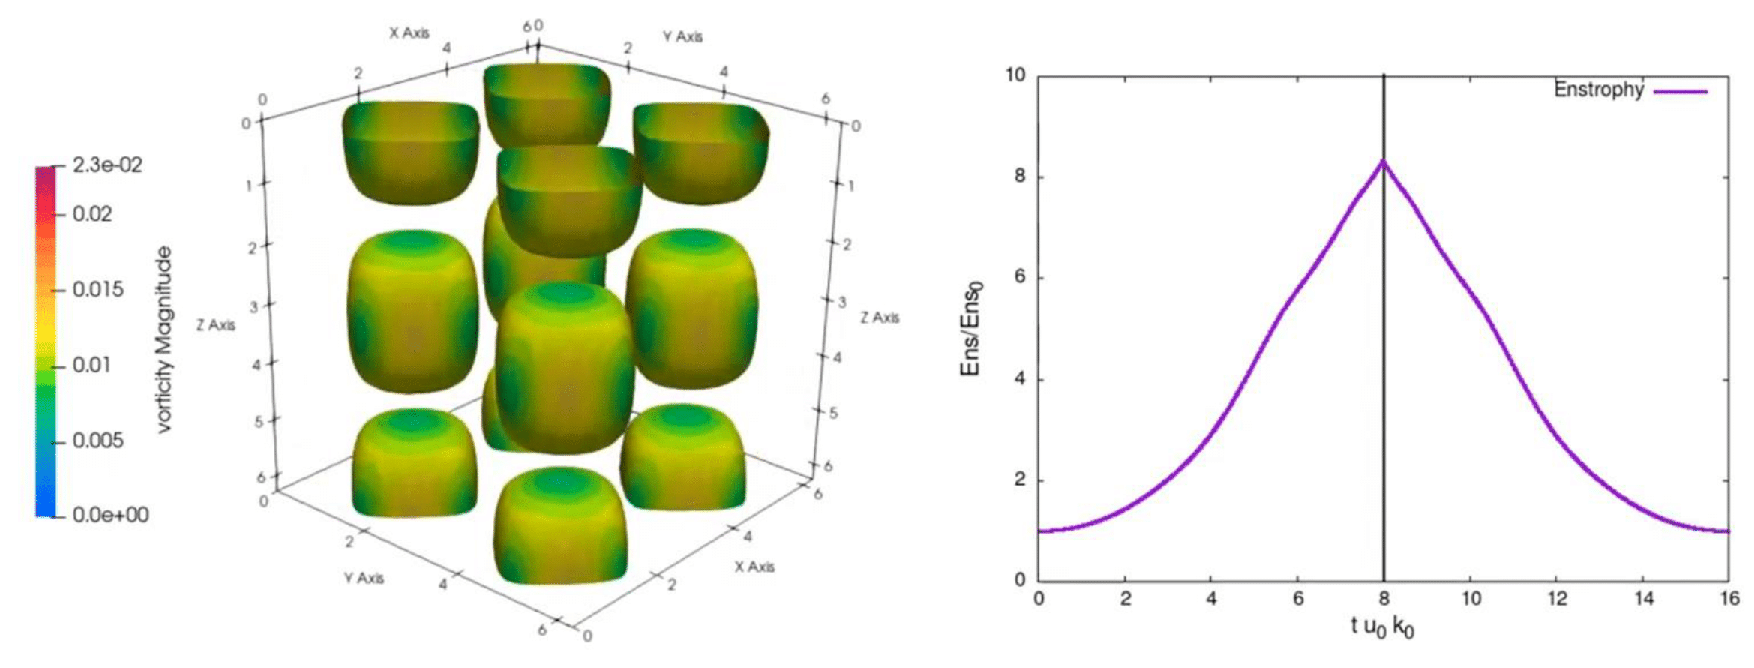
\includegraphics[width=0.99\linewidth]{TGV}
		\caption{A destra il plot della velocità graficata mediante il Q-criterion del Taylor-Green Vortex, sulla sinistra il grafico dell'Enstrofia che, dopo aver invertito il campo di velocità al tempo adimensionalizzato 8, recupera l'andamento fino alle raggiungimento delle condizioni iniziali. Il tempo adimensinalizzato è calcolato com $t u_0 k_0$ dove $k_0$ è il numero d'onda.}
		\label{TGV}
	\end{figure} 
	
	\subsection{Forward Step}
	Lo studio del flusso non viscoso su un gradino rivolto in avanti è stato originariamente proposto da \cite{EMERY1968306} per confrontare gli schemi di cattura dello shock. In questo caso è stato utilizzato per analizzare il comportamento di rhoEnergyFOAM su flussi supersonici in presenza di urti. 
	Il flusso supersonico a M = 3 affronta un gradino di altezza $0.2 h$, dove $h$ è l'altezza del canale. La lunghezza totale del canale è $3 h$, il bordo anteriore del gradino è a $0.6 h$ dall'ingresso e la mesh è uniforme, con $N_x \times N_y = 240 \times 80$ celle nelle direzioni delle coordinate. Le condizioni al contorno di scorrimento sono imposte alle pareti superiore e inferiore e tutte le variabili sono estrapolate all'uscita. Per questo caso il test viene eseguito in modalità C. L'ispezione del modello di shock mostra che, nonostante le somiglianze qualitative, rhoEnergyFOAM fornisce dettagli di flusso aggiuntivi che sono appena visibili con rhoCentralFOAM. In particolare la linea di scivolamento che esce dal punto quadruplo vicino alla parete superiore è evanescente in rhoCentralFOAM, a causa della sua maggiore diffusione numerica.
	
	\subsection{Onera M6}
	Questo caso mira alla valutazione di un flusso inviscido intorno all'ala dell'Onera M6, il cui flusso è transonico con numero di Mach $M = 0.8395$, e l'angolo di attacco è $\alpha = 3.06^\circ$ . \'E stata utilizzata una mesh non strutturata che include 341'797 celle tetraedriche, all'interno di una scatola computazionale esterna di dimensioni $L_x \times L_y \times L_z = 10c \times 10c \times 5c$, dove c è la corda nella sezione della radice dell'ala. Le simulazioni numeriche sono state effettuate utilizzando sia rhoCentralFOAM che rhoEnergyFOAM in modo C.
	
	\subsection{RANS and DES of a flow past circular cylinder}
	Il flusso turbolento attorno a un cilindro circolare è stato studiato numericamente per mezzo di rhoEnergyFOAM in modalità B, sia attraverso la URANS (Unsteady Reynolds-Averaged Navier-Stokes) che con la simulazione DES (Detached Eddy Simulation), basandosi sul classico modello di turbolenza di Spalart-Allmaras e la sua estensione DES, rispettivamente. Il numero di Mach del flusso libero è $M_0 = u_0 /c_0 = 0.1$, dove $u_0$ e $c_0$ sono la velocità del flusso libero e la velocità del suono, e il Reynolds basato sul diametro del cilindro è $Re_D = \rho_0 u_0 D/ \mu_w$, con $\rho_0$ la densità del flusso libero e $\mu_w$ la viscosità della parete. Una mesh di tipo O viene utilizzata per DES con $Nr \times N_\theta \times N_z = 256 \times 256 \times 48$ celle con tangente iperbolica che si estende verso il muro in un dominio $L_r \times L_z = 20D \times 2D$, mentre viene utilizzata la stessa mesh con $N_z = 1$ per la URANS. I risultati sono ancora in fase di discussione.
	
	\subsection{Bachalo-Johnson}
	Il caso in questione studia il flusso transonico sul dosso assialsimmetrico di Bachalo-Johnson. La lunghezza del dosso è c = 20.32 cm. Il dominio è costituito da un cuneo di $1^\circ$ con raggio interno $r_{in}/c = 0.375$ e raggio esterno $r_{out}/c = 4.0$. L'altezza del dosso è $h/c = 0.09375$. La condizione a contorno è di no-slip vicino alla parete. All'inlet la velocità, la temperatura totale e la pressione totale sono costanti ("fixed-value"), mentre all'outlet la velocità, la temperatura e la pressione sono impostate con uno "zero-gradient". I confini su entrambi i lati del dominio computazionale sono periodici, cioè è stata decisa la condizione "cyclic" di OpenFOAM per rendere la simulazione 3D e assialsimmetrica. I risultati sono ancora in fase di discussione.
	
	\subsection{RAE-2822}
	Il flusso transonico intorno al profilo alare RAE-2822 è stato simulato tramite RANS, utilizzando il modello standard di Spalart-Allmaras. Il numero di Mach è $M = 0.729$, il numero di Reynolds della corda è $Re_c = \rho_0 u_0 c /\mu_0 = 6.5 \times 10^6$, e l'angolo di attacco è $\alpha = 2.31^\circ$. \'E stata utilizzata una mesh strutturata di tipo C che comprende $369 \times 256$ celle, con tangente iperbolica che si estende verso la parete. Il limite del "far-field" si trova a circa 20 corde dalla parete, dove le condizioni al contorno di ingresso/uscita sono imposte, mentre le condizioni al contorno isotermiche di non slittamento sono imposte alla parete del profilo alare.
	
	\subsubsection{Taylor-Green Vortex}
	Il Taylor-Green vortex illustra il meccanismo di base del decadimento della produzione di piccoli vortici detti \say{eddies}. Il caso studio dimostra le proprietà di conservazione dell'energia cinetica del solutore rhoEnergyFOAM. Sono state effettuate prove sia con rhoEnergyFOAM che con rhoCentralFOAM, prima su una mesh strutturata con $32^3$ celle e poi su una mesh non strutturata con 85'056 prismi. Tale mesh è stata realizzata con Gmsh, estrudendo gli elementi triangolari di una faccia lungo la terza direzione principale. Per valutare la conservazione della TKE (Turbulent Kinetic Energy) è stata effettuata l'inversione del tempo a metà della simulazione, verificando effettivamente se la soluzione tornasse ai valori delle condizioni iniziali. Per una migliore visualizzazione dei risultati, è stato realizzato un video in cui si possono apprezzare contemporaneamente le simulazioni ottenute con Paraview e i grafici animati in cui viene rappresentatato l'andamento dell'enstrofia. In figura \ref{TGV_Qcriterion} viene mostrato il campo di velocità del Taylor-Green vortex visualizzato con il  Q-criterion, mentre in figura \ref{TGV_Enstrophy} si può apprezzare il grafico dell'enstrofia ottenuto con rhoEnergyFOAM che, dopo aver invertito il campo di velocità al tempo adimensionalizzato $t^*=8$, recupera l'andamento fino alle raggiungimento delle condizioni iniziali. Il tempo adimensinalizzato è calcolato con $t^* = t u_0 k_0$.
	
	\begin{figure}[htp]
		\centering
		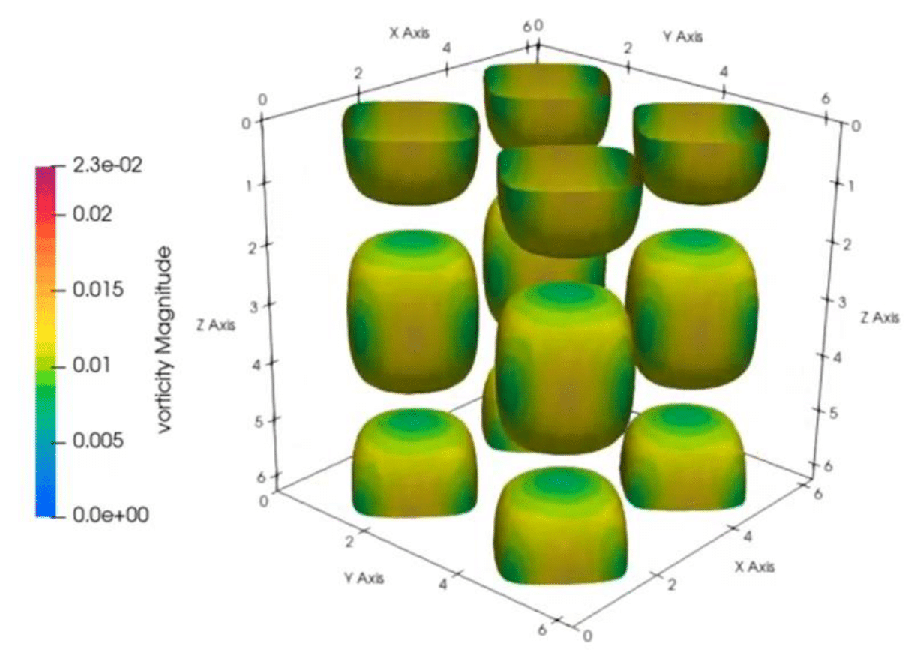
\includegraphics[width=0.66\linewidth]{TGV_Qcriterion}
		\caption{Campo di velocità del Taylor-Green Vortex graficata mediante il Q-criterion.}
		\label{TGV_Qcriterion}
	\end{figure} 
	
	\begin{figure}[htp]
		\centering
		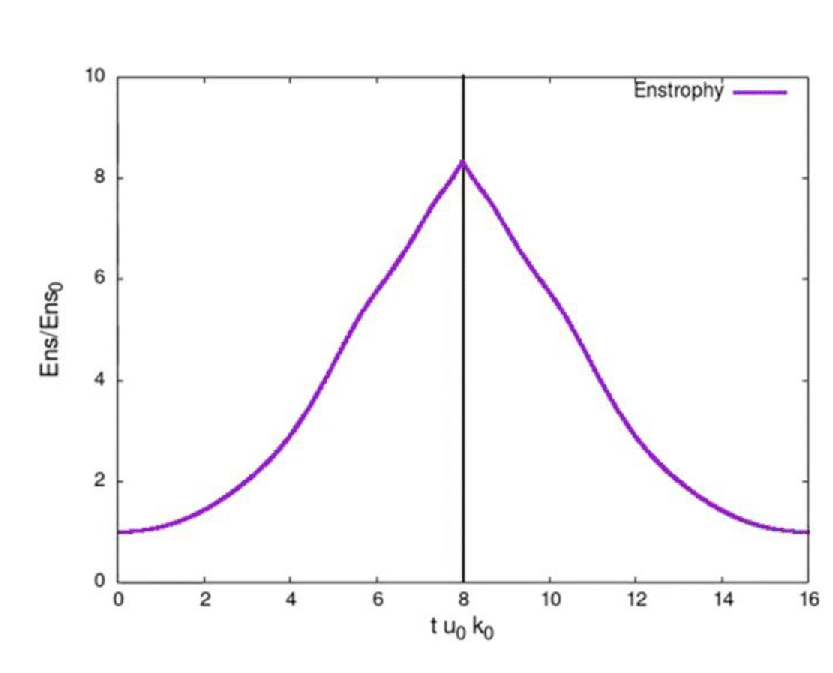
\includegraphics[width=0.66 \linewidth]{TGV_Enstrophy}
		\caption{Grafico dell'enstrofia ottenuto con rhoEnergyFOAM. Il tempo adimensinalizzato è calcolato con $t u_0 k_0$, dove $t$ è il tempo fisico, $u_0$ è la velocità all'infinito e $k_0$ è il numero d'onda.}
		\label{TGV_Enstrophy}
	\end{figure} 
	
	\newpage
	
	\subsubsection{Forward Step}
	Lo studio del flusso non viscoso su un gradino rivolto in avanti è stato originariamente proposto da \citet{EMERY1968306} per confrontare gli schemi di cattura dello shock. In questo caso è stato utilizzato per analizzare il comportamento di rhoEnergyFOAM su flussi supersonici in presenza di urti. 
	Il flusso supersonico a numero di Mach M = 3 affronta un gradino di altezza $0.2 h$, dove $h$ è l'altezza del canale. La lunghezza totale del canale è $3 h$, il bordo anteriore del gradino è a $0.6 h$ dall'ingresso e la mesh è uniforme, con $N_x \times N_y = 240 \times 80$ celle nelle direzioni delle coordinate. Le condizioni al contorno di scorrimento sono imposte alle pareti superiore e inferiore e tutte le variabili sono estrapolate all'uscita. Per questo caso il test è stato eseguito in modalità C. L'ispezione del modello di shock mostra che, nonostante le somiglianze qualitative, rhoEnergyFOAM fornisce dettagli di flusso aggiuntivi che sono appena visibili con rhoCentralFOAM. In particolare la linea di scivolamento che esce dal punto quadruplo vicino alla parete superiore è evanescente in rhoCentralFOAM, a causa della sua maggiore diffusione numerica.
	
	\begin{figure}[htp]
		\centering
		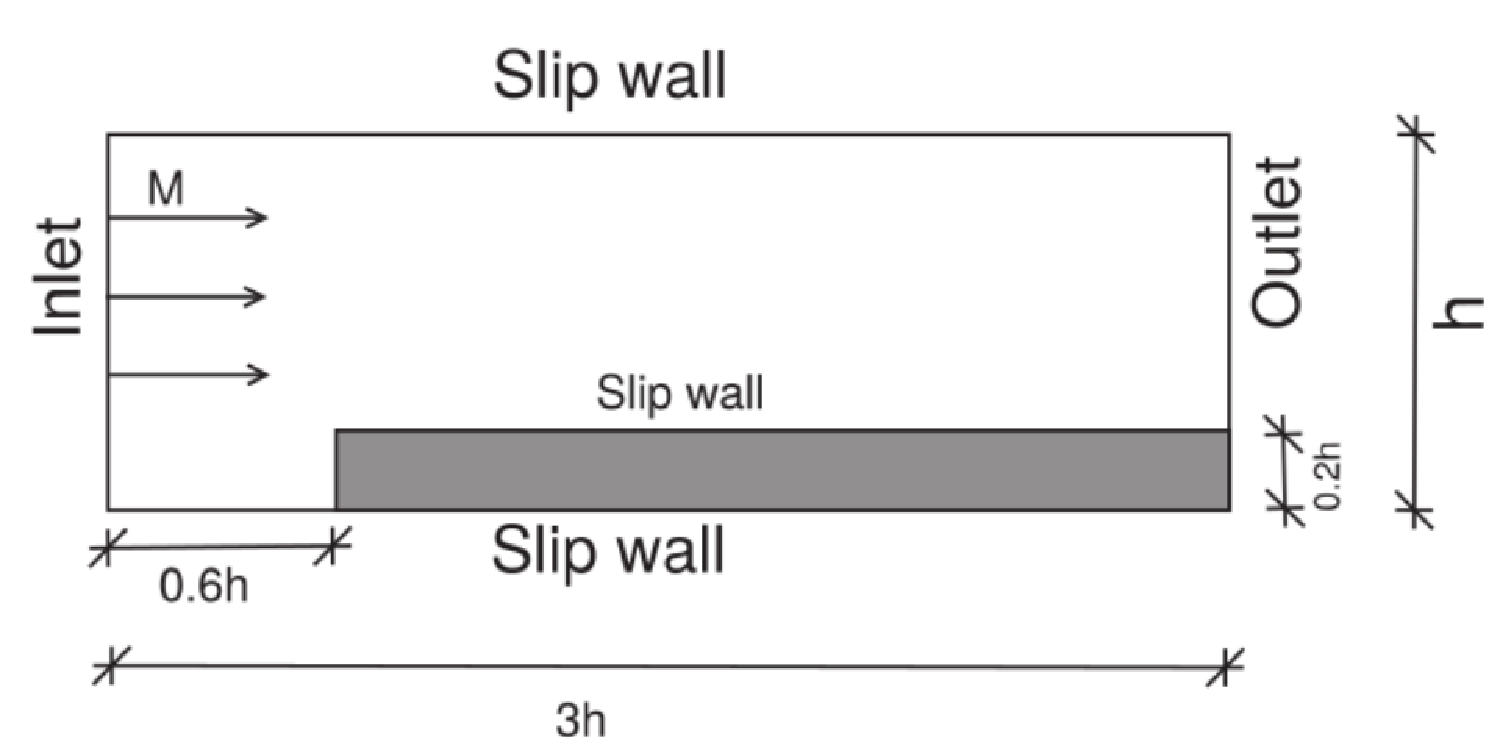
\includegraphics[width=0.94 \linewidth, height=0.26\textheight]{FS}
		\caption{geometria del Forward Step e condizioni al contorno}
		\label{FS}
	\end{figure} 
	\begin{figure}[htp]
		\centering
		\subfloat
		{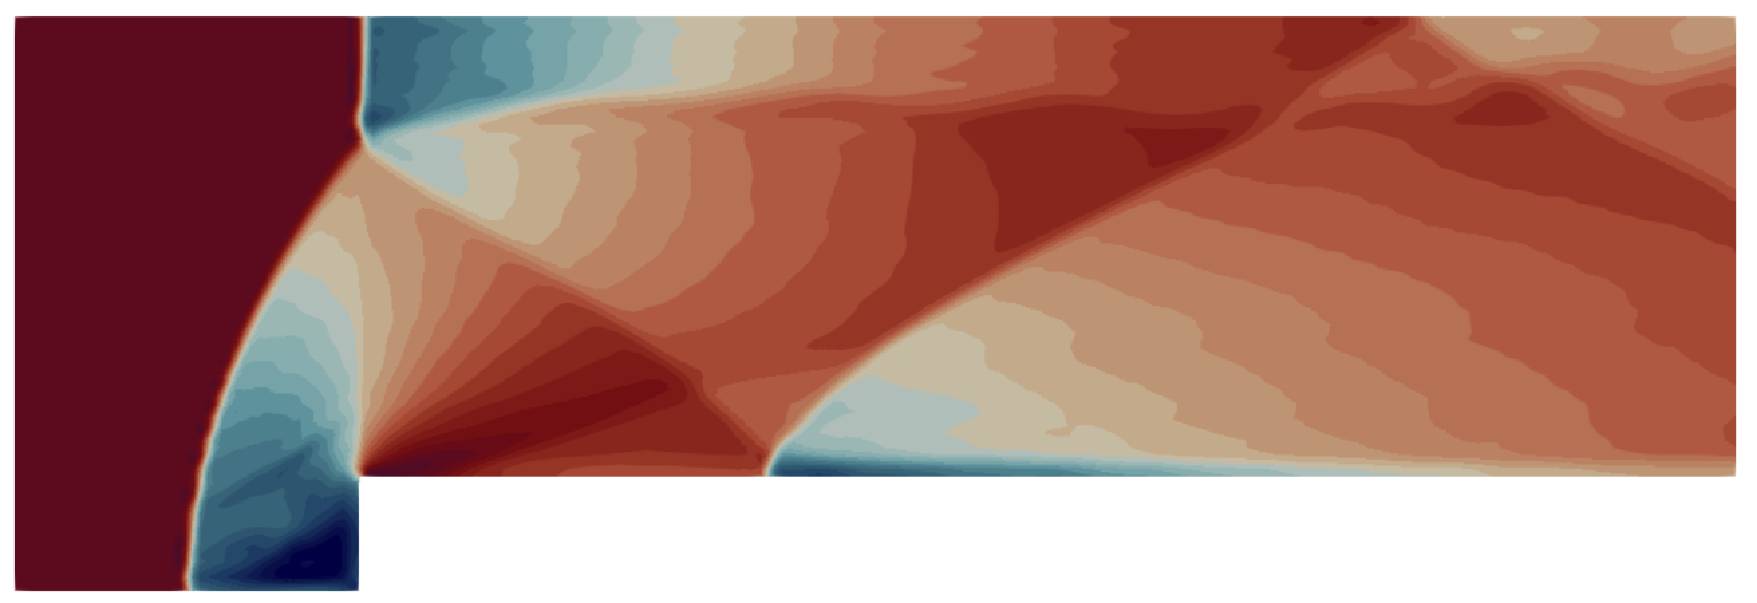
\includegraphics[width=0.7\textwidth]{FS_velocity}} \quad 
		\subfloat
		\centering
		{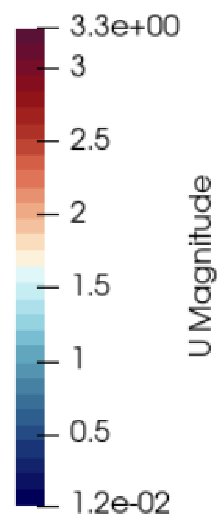
\includegraphics[width=0.1\textwidth, height=0.16\textheight]{FS_velocitybar}}
		\caption{campo di velocità supersonico del Forward Step raggiunto a Mach 3.}
		\label{fig:FS}
	\end{figure}
	
	\subsubsection{Onera M6 inviscid}
	Questo caso mira alla valutazione di un flusso inviscido intorno all'ala dell'Onera M6, il cui flusso è transonico con numero di Mach $M = 0.8395$, e l'angolo di attacco è $\alpha = 3.06^\circ$. \'E stata utilizzata una mesh non strutturata che include 341'797 celle tetraedriche, all'interno di una scatola computazionale esterna di dimensioni $L_x \times L_y \times L_z = 10c \times 10c \times 5c$, dove c è la corda nella sezione della radice dell'ala. Le simulazioni numeriche sono state effettuate utilizzando sia rhoCentralFOAM che rhoEnergyFOAM in modo C, confrontando i risultati anche con i valori dei dati sperimentali.
	
	\begin{figure}[htp]
		\centering
		{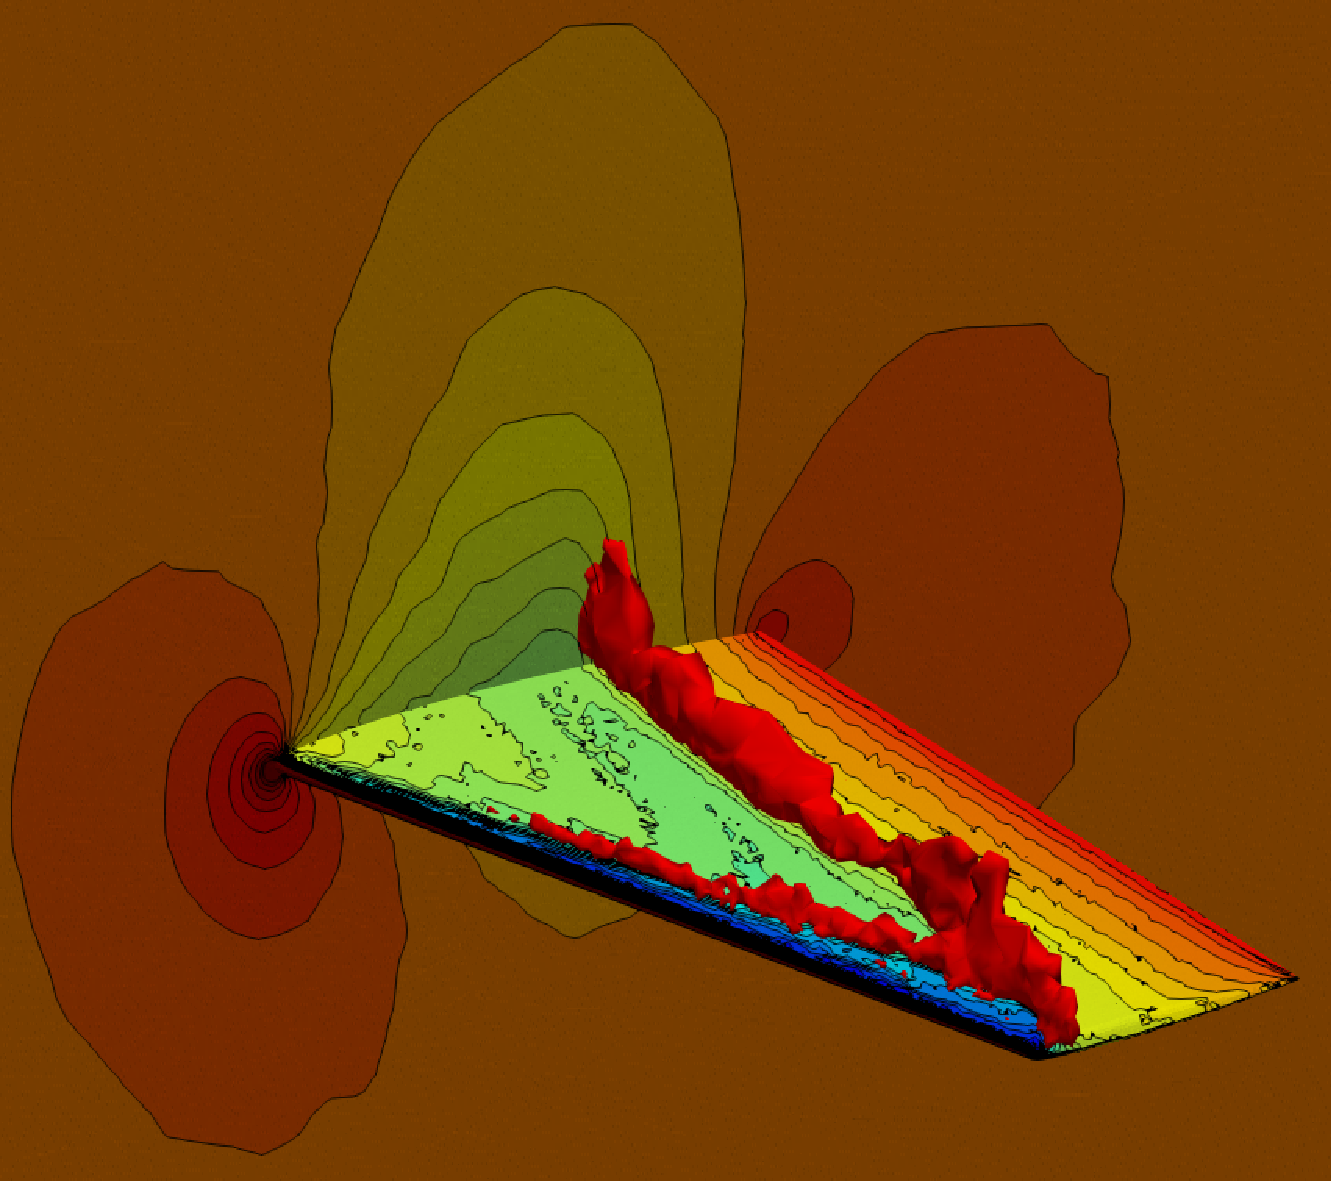
\includegraphics[width=0.65\linewidth, height=0.32\textheight]{Ducros}}  
		\centering
		{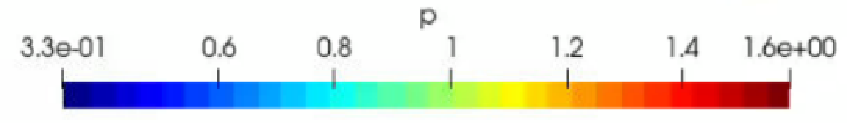
\includegraphics[width=0.6\linewidth]{Ducros_bar}}
		\caption{Campo di pressione dell'Onera M6 con sovrapposta l'isosuperficie del sensore di Ducros che evidenzia la presenza di due onde d'urto.}
		\label{OneraM6_pressurefield}
	\end{figure}
	
	\begin{figure}[htp]
		\centering
		{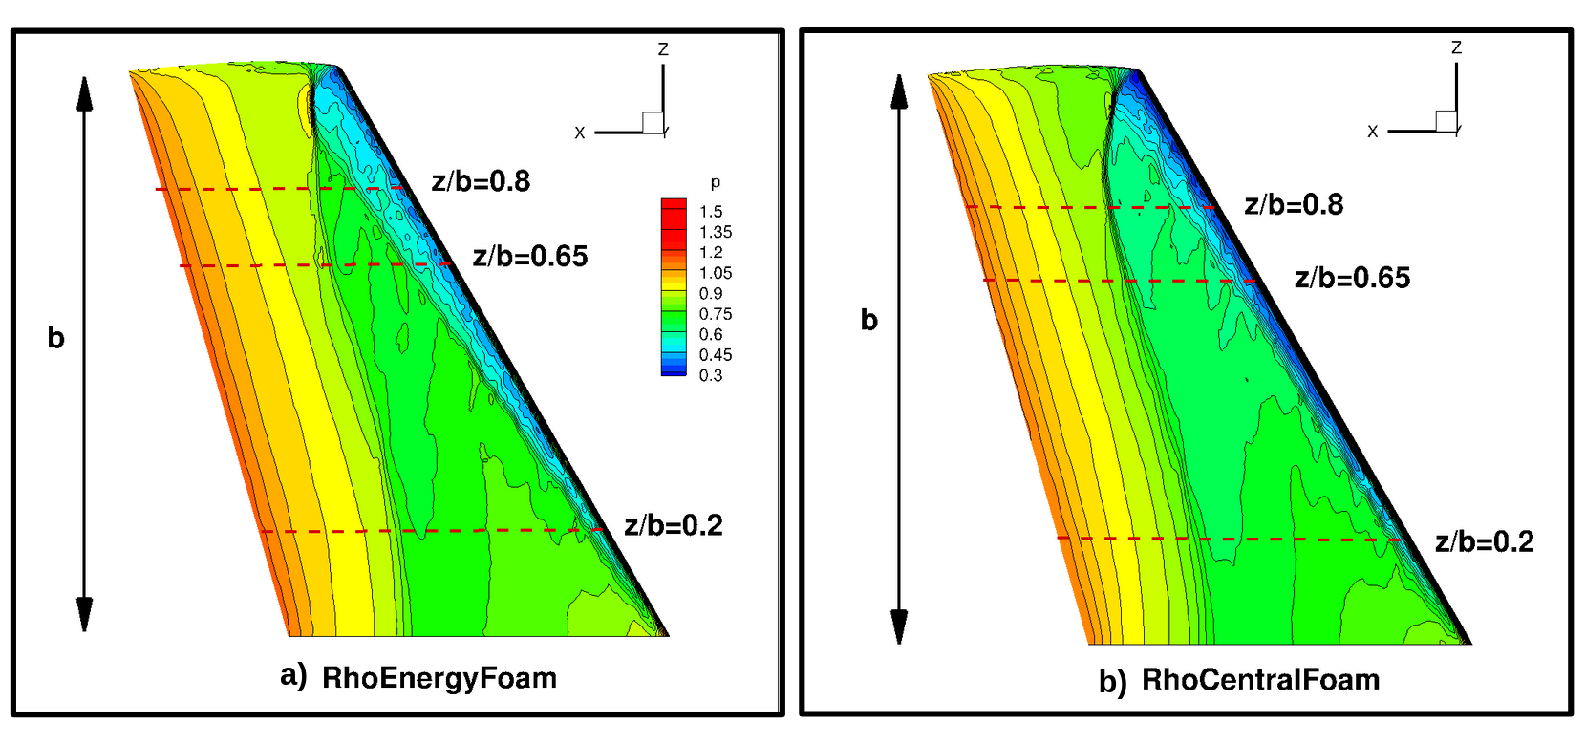
\includegraphics[width=0.95\linewidth]{Cp_contours_oneram6_1}}  
		\caption{Flusso attorno all'ala dell'ONERA M6: profili di pressione calcolati sulla superficie dell'ala per rhoEnergyFoam (a) e rhoCentralFoam (b). Nell'intervallo $0.3 < p/p_\infty < 1.5$ sono mostrati 32 livelli  (scala di colori dal blu a rosso). Le linee tratteggiate indicano le sezioni alari utilizzate nella Figura \ref{Cp_oneraM6}}
		\label{Cp_contours_oneraM6}
	\end{figure}
	
	La figura \ref{OneraM6_pressurefield} mostra il campo di pressione calcolato usando rhoEnergyFoam con sovrapposta l'isosuperficie del sensore d'urto, che evidenzia la presenza di due onde d'urto, una primaria all'incirca a metà della corda e una secondaria vicino al bordo d'attacco, che alla fine si uniscono vicino alla punta dell'ala. La figura \ref{Cp_contours_oneraM6} mostra il campo di pressione calcolato sulla superficie di aspirazione dell'ala per rhoEnergyFoam (figura \ref{Cp_contours_oneraM6}a) e rhoCentralFoam (figura \ref{Cp_contours_oneraM6}b), che evidenzia le differenze qualitative tra i due solutori. Sebbene le caratteristiche principali del flusso siano colte da entrambi i solutori, sembra che lo shock di bordo sia molto più debole in rhoCentralFoam e che lo shock primario sia molto più spesso, soprattutto verso la radice dell'ala, a causa della natura diffusiva del solutore. Una valutazione più quantitativa viene effettuata nella figura \ref{Cp_oneraM6}, dove si confrontano le distribuzioni calcolate del coefficiente di pressione con i dati sperimentali di Schmitt e Charpin \citep{schmitt1979pressure}, in corrispondenza delle quattro sezioni alari indicate con le linee tratteggiate nella figura \ref{Cp_contours_oneraM6}. Nella sezione più interna (pannello a) lo shock primario è piuttosto debole e appena evidente in rhoCentralFoam, mentre rhoEnergyFoam fornisce una previsione favorevole sia della forza che della posizione dello shock. Nelle sezioni intermedie (pannelli b,c) sono presenti entrambi gli shock, che sono di nuovo correttamente catturati da rhoEnergyFoam, mentre rhoCentralFoam mostra un'eccessiva sbavatura. Nella sezione più esterna (pannello d) lo shock primario e quello secondario si fondono in un unico shock più forte, la cui ampiezza è ben catturata da rhoEnergyFoam. 
	
	\begin{figure}[htp]
		\begin{center}
			{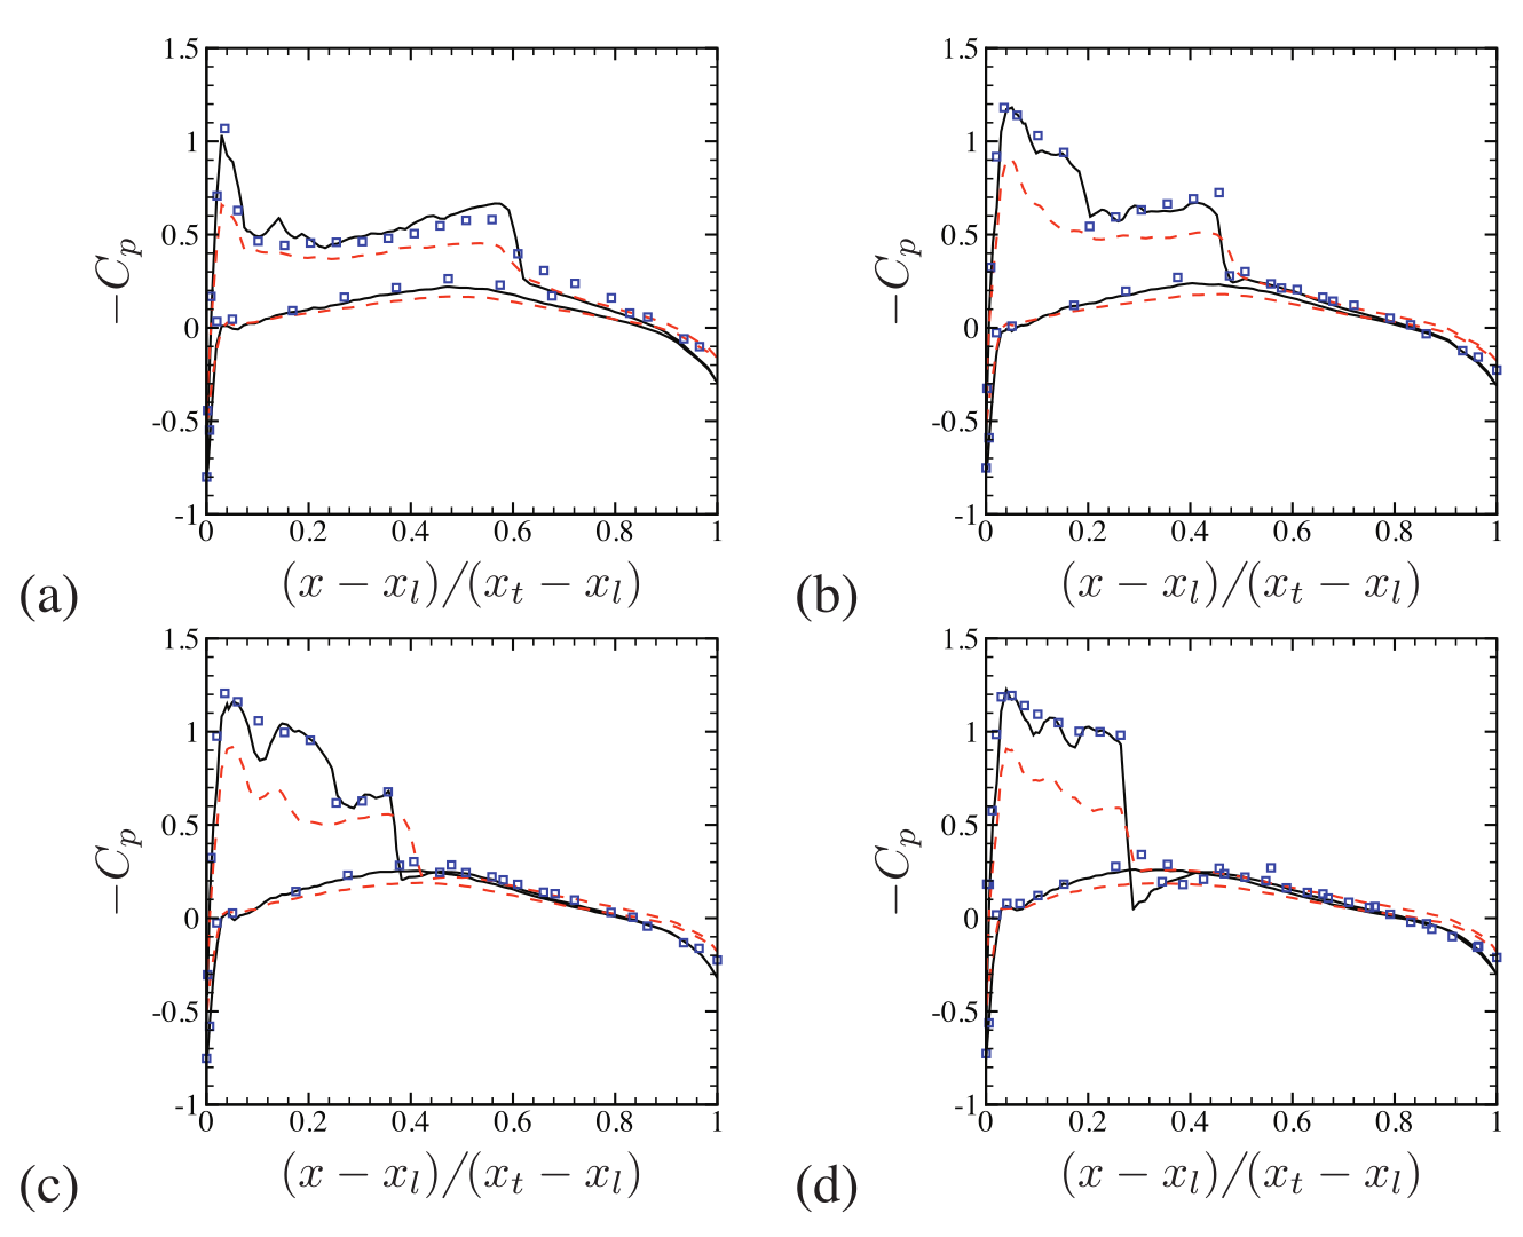
\includegraphics[width=0.95\linewidth]{Cp_oneram6}}  
			\caption{Flusso attorno all'ala ONERA M6: coefficiente di pressione $(Cp = (p-p_\infty)/(\dfrac{1}{2}\rho_\infty u^2_\infty))$ a varie sezioni dell'ala (vedi Fig. \ref{Cp_contours_oneraM6}): (a) $z/b = 0.2$, (b) $z/b = 0.65$, (c) $z/b = 0.8$, (d) $z/b = 0.9$, per rhoEnergyFoam (linea continua) rhoCentralFoam (linea tratteggiata) e dati sperimentali (simboli quadrati). $x_l$ e $x_t$ indicano rispettivamente le coordinate del bordo d'attacco e del bordo d'uscita di ciascuna sezione alare.}
			\label{Cp_oneraM6}
		\end{center}
	\end{figure}
	
	\newpage
	
	\subsubsection{RANS and DES of a flow past circular cylinder}
	Il flusso turbolento attorno a un cilindro circolare è stato studiato numericamente per mezzo di rhoEnergyFOAM in modalità B, sia attraverso la URANS (Unsteady Reynolds-Averaged Navier-Stokes) che con la simulazione DES (Detached Eddy Simulation), basandosi sul classico modello di turbolenza di Spalart-Allmaras e la sua estensione DES, rispettivamente. Il numero di Mach del flusso libero è $M_\infty = u_\infty /c_\infty = 0.1$, dove $u_\infty$ e $c_\infty$ sono la velocità del flusso libero e la velocità del suono, e il Reynolds basato sul diametro del cilindro è $Re_D = \rho_\infty u_\infty D/ \mu_w$, con $\rho_\infty$ la densità del flusso libero e $\mu_w$ la viscosità della parete. Una mesh di tipo O viene utilizzata per DES con $Nr \times N_\theta \times N_z = 256 \times 256 \times 48$ celle con tangente iperbolica che si estende verso il muro in un dominio $L_r \times L_z = 20D \times 2D$, mentre viene utilizzata la stessa mesh con $N_z = 1$ per la URANS.
	La griglia è allungata verso il cilindro con il primo punto della griglia fuori dalla parete a $y_+ \approx 150 - 200$, quindi ci affidiamo all'uso di funzioni di parete per un corretto trattamento della parete. In particolare, si utilizza la legge di equilibrio della parete di Spalding \citep{spalding1961single}. Le condizioni al contorno isotermiche di \say{no-slip} sono imposte alla parete, mentre le condizioni al contorno \say{fixedValue} e/o \say{zeroGradient} sono utilizzate per tutte le variabili all'ingresso e all'uscita, rispettivamente, con la viscosità turbolenta impostata a $\mu_{t0} = 3\mu_w$. I risultati numerici sono confrontati con precedenti simulazioni numeriche ed esperimenti. La principale differenza rispetto a questi ultimi è l'assenza di vorticità sensibile nella URANS che è probabilmente da ricondurre all'uso di funzioni di parete. Lo shedding è osservato nella DES in figura \ref{Des_Cylinder}, con parametri globali di flusso in ragionevole accordo con altre fonti. Il coefficiente di pressione di parete e i profili di velocità media nella scia del cilindro sono ulteriormente analizzati nelle figure \ref{Cp_Cylinder} e \ref{Cylinder}. Il confronto è complessivamente soddisfacente sia per il coefficiente di pressione che per i profili di velocità, con la differenza principale che si osserva una scia cilindrica più lunga nella URANS rispetto alle simulazioni numeriche di riferimento di Catalano \citep{Catalano}. Anche in questo caso, questa deviazione può essere dovuta a una previsione imprecisa del punto di separazione causata da un trattamento approssimativo delle pareti.
	
	\begin{figure}[htp]
		\begin{center}
			{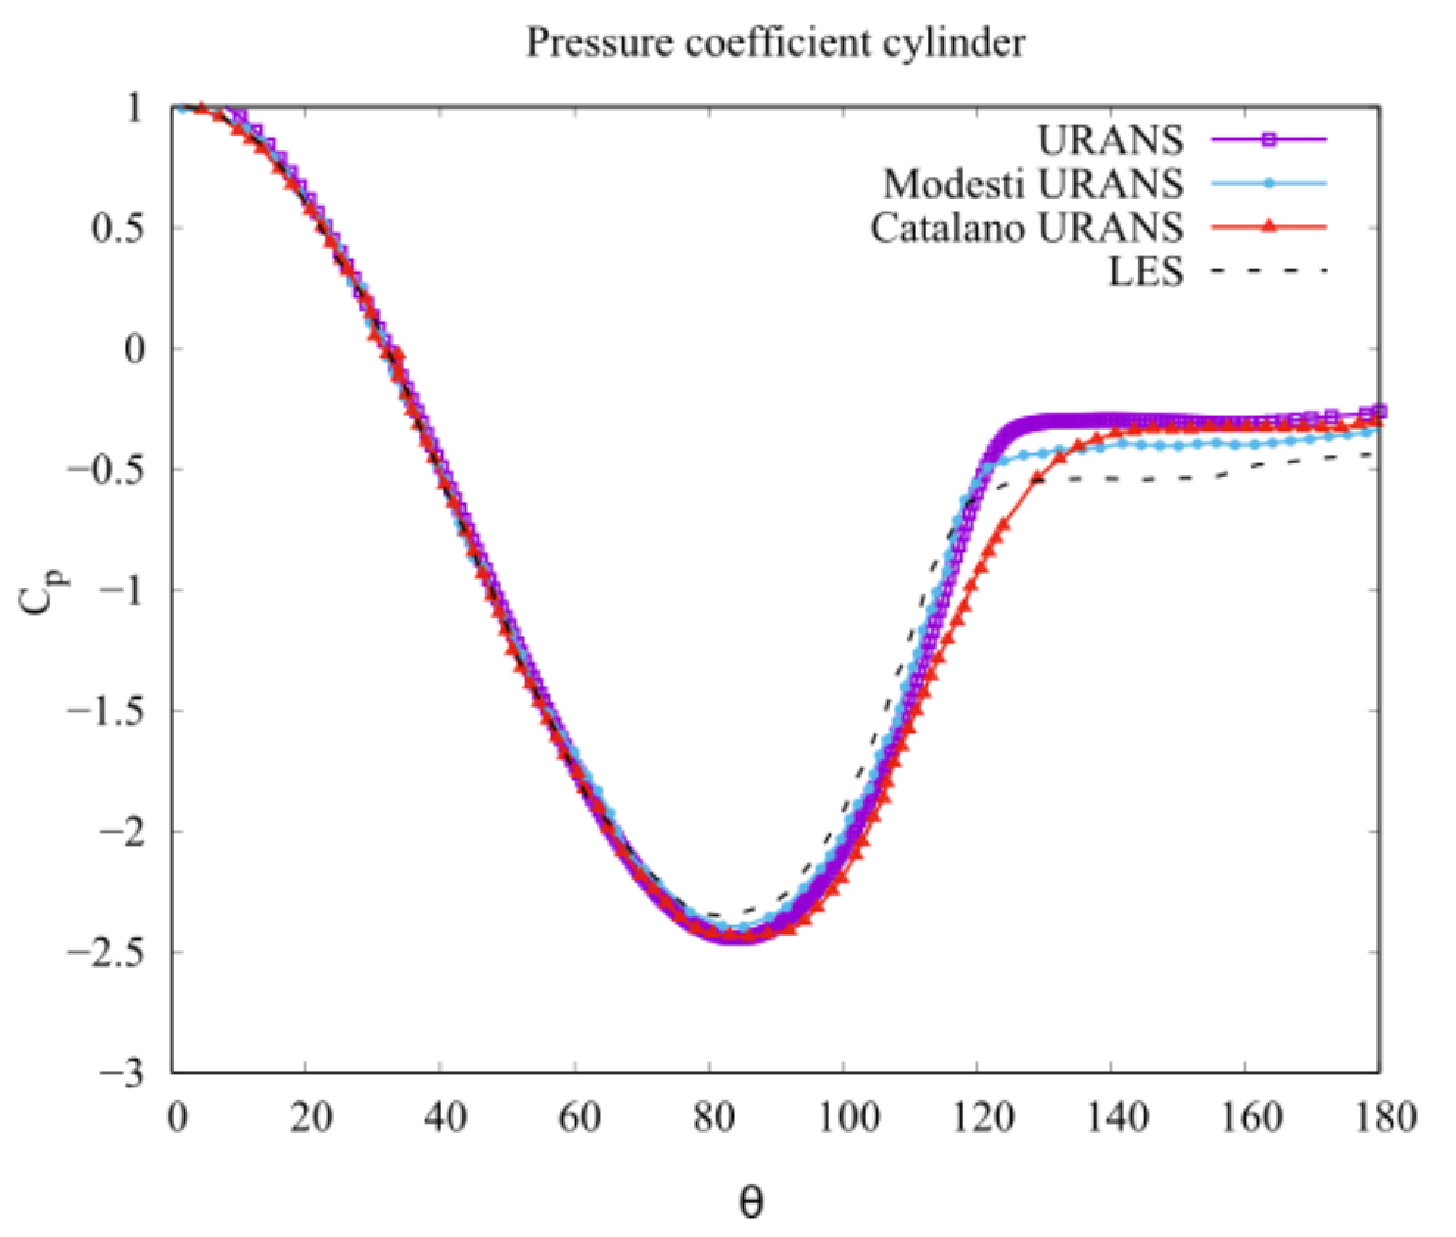
\includegraphics[width=0.579\linewidth]{pressure_coeff_cylinder}}  
			\caption{Simulazione numerica del flusso attorno a un cilindro circolare: coefficiente di pressione ottenuto da rhoEnergyFoam in modalità B con URANS (linea viola continua e quadrati) confrontato con URANS di Modesti(linea celeste) e LES (tratteggiato) di Catalano et al. \cite{Catalano}}
			\label{Cp_Cylinder}
		\end{center}
	\end{figure}
	
	\begin{figure}[htp]
		\centering
		\subfloat
		{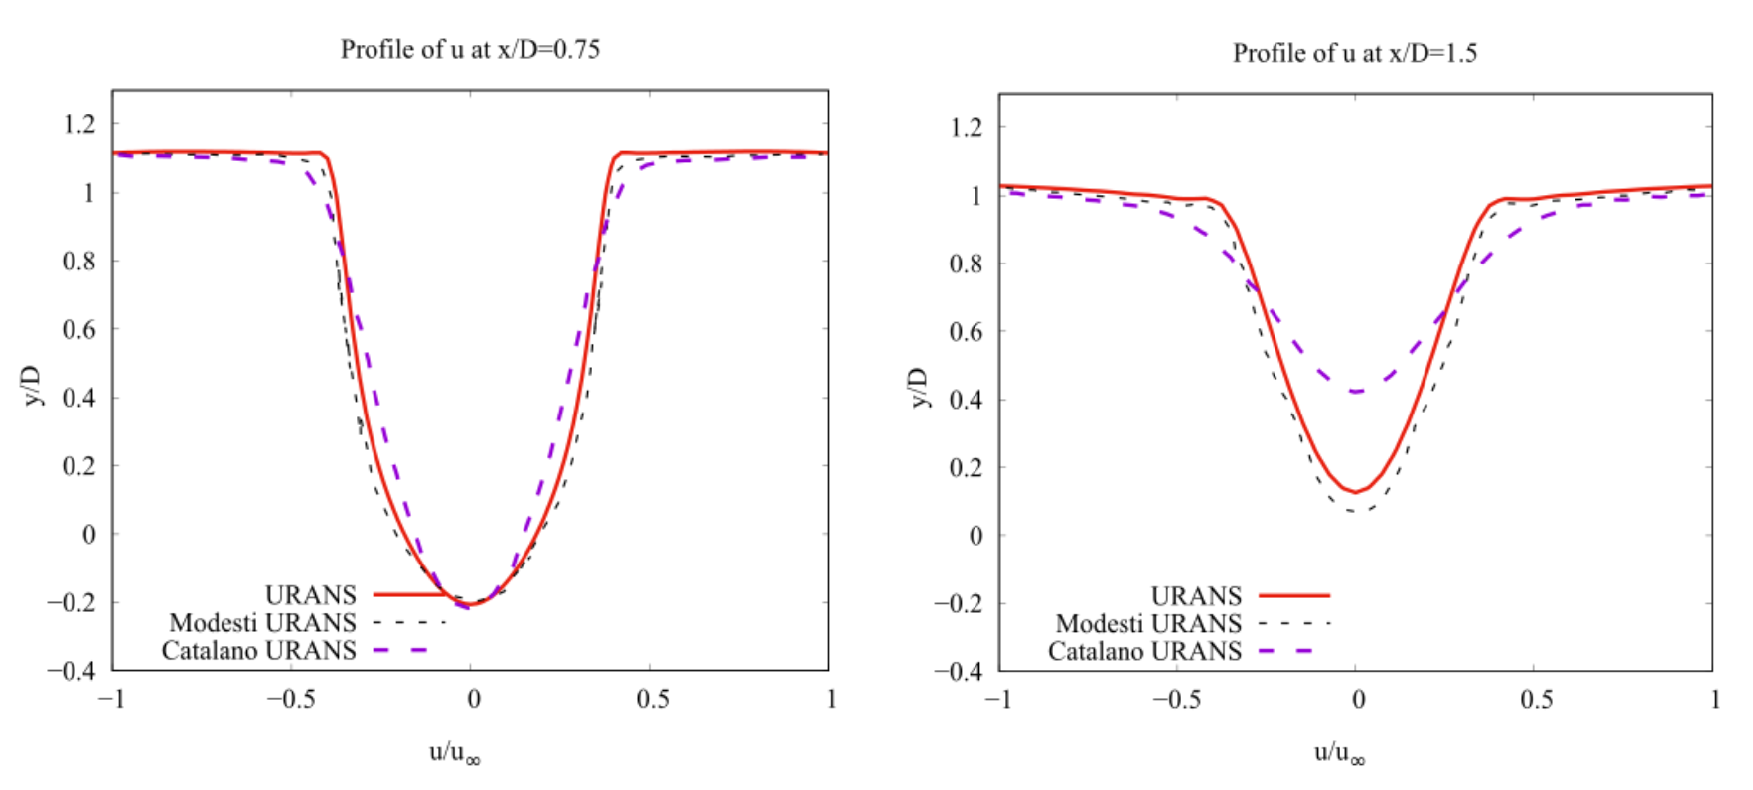
\includegraphics[width=0.9\textwidth, height=0.27\textheight]{Cylinder_u.pdf}} \quad 
		\subfloat
		\centering
		{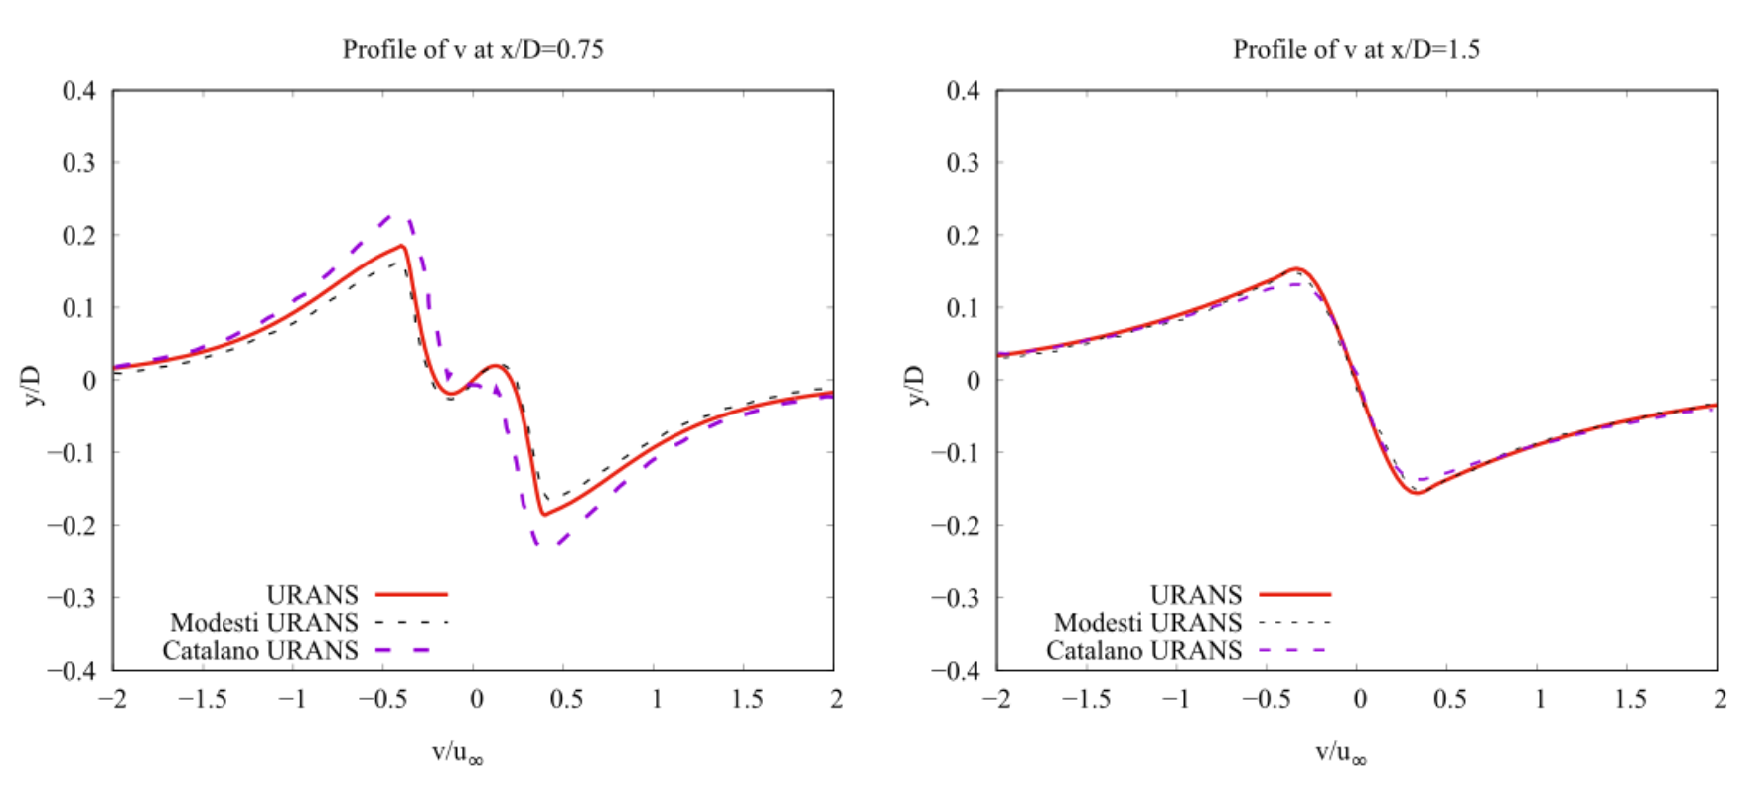
\includegraphics[width=0.9\textwidth, height=0.27\textheight]{Cylinder_v}}
		\caption{Simulazione numerica del flusso attorno a un cilindro circolare: profili di velocità media a $x/D = 0.75$ e $x/D = 1.5$ per la URANS (linea rossa), la URANS di Modesti (linea tratteggiata viola sottile) rispetto alla URANS (linea tratteggiata viola spessa) di Catalano.}
		\label{Cylinder}
	\end{figure}
	
	\begin{figure}[htp]
		\begin{center}
			{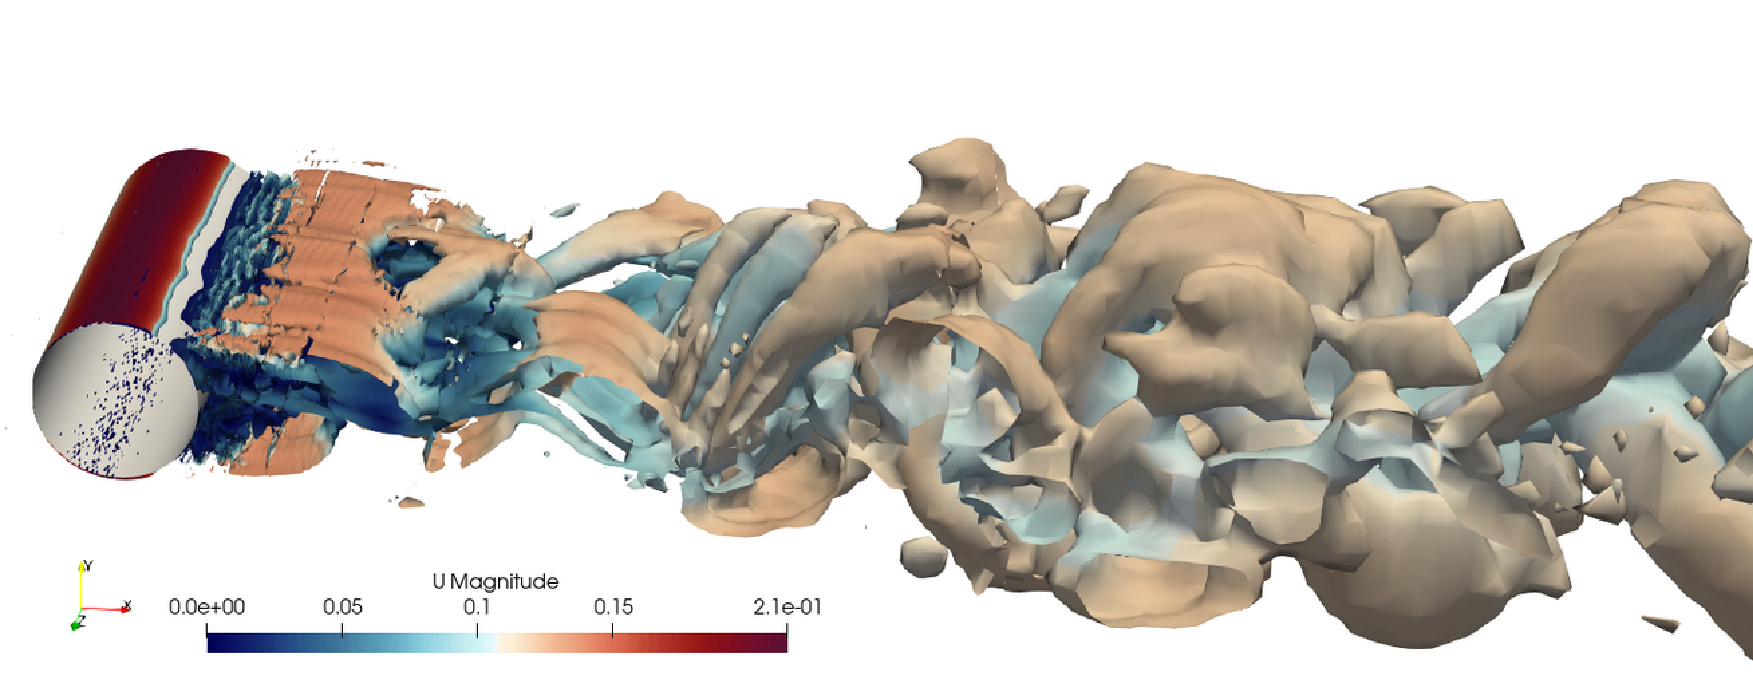
\includegraphics[width=0.98\linewidth]{Des_cylinder}}  
			\caption{DES del flusso 3D attorno a un cilindro circolare: rappresentazione del campo di velocità mediante il Q-criterion $Q = \dfrac{1}{2} [(\nabla \cdot u)^2 - \nabla u : \nabla u^T]$.}
			\label{Des_Cylinder}
		\end{center}
	\end{figure}
	
	\subsubsection{RAE-2822}
	Il flusso transonico intorno al profilo RAE-2822 è stato simulato tramite RANS, utilizzando il modello standard di Spalart-Allmaras. Il numero di Mach è $M = 0.729$, il numero di Reynolds della corda è $Re_c = \rho_0 u_0 c /\mu_0 = 6.5 \times 10^6$, e l'angolo di attacco è $\alpha = 2.31^\circ$. \'E stata utilizzata una mesh strutturata di tipo C che comprende $369 \times 256$ celle, con tangente iperbolica che si estende verso la parete. Il limite del \say{farfield} si trova a circa 20 corde dalla parete, dove le condizioni al contorno di ingresso/uscita sono imposte, mentre le condizioni al contorno isotermiche di non slittamento sono imposte alla parete del profilo alare. I campi di pressione calcolati sono confrontati nella figura \ref{RAE2822_pressurefield}, che mostra la presenza di un singolo shock normale sul lato di aspirazione e differenze minime tra i due solutori. Il confronto dettagliato dei coefficienti di pressione con gli esperimenti di \citet{cook1977aerofoil} e le simulazioni \cite{slater2010rae2822}, mostrato in figura \ref{Cp_RAE2822}, è soddisfacente per entrambi i solutori, anche se in questo caso rhoCentralFoam sembra essere più vicino agli esperimenti e rhoEnergyFoam più vicino alle simulazioni precedenti.
	
	\begin{figure}[htp]
		\centering
		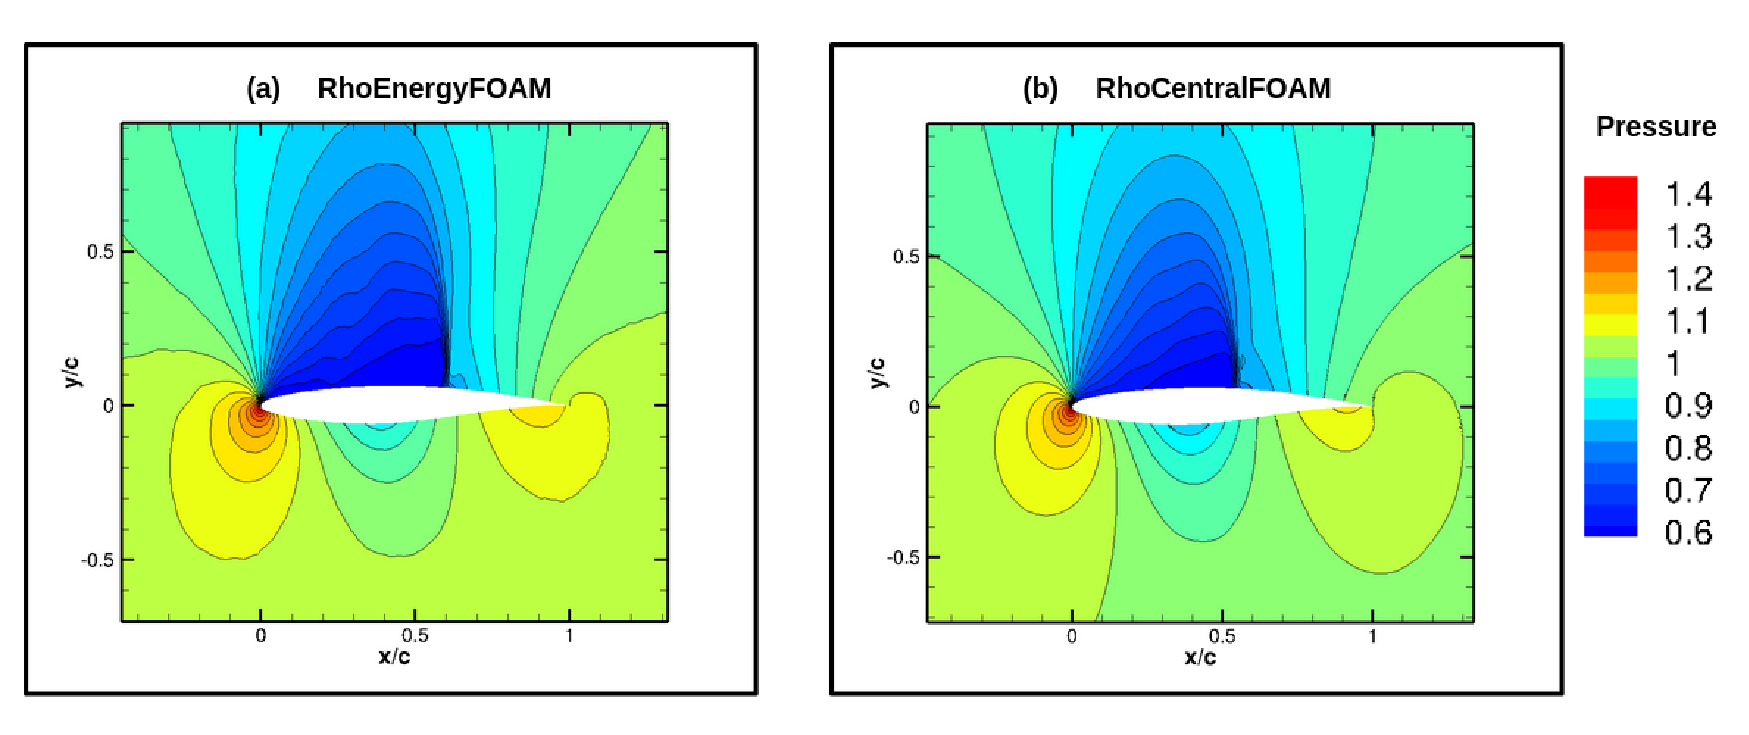
\includegraphics[width=0.9\textwidth]{RAE2822_pressurefield}
		\caption{RANS del RAE2822: Campi di pressione calcolai da rhoEnergyFoam (a) e rhoCentralFoam (b). Nella rappresentazione sono stati utilizzati 24 livelli nel range $0.6 < p/p_\infty < 1.4$.}
		\label{RAE2822_pressurefield}
	\end{figure}
	
	\begin{figure}[htp]
		\centering
		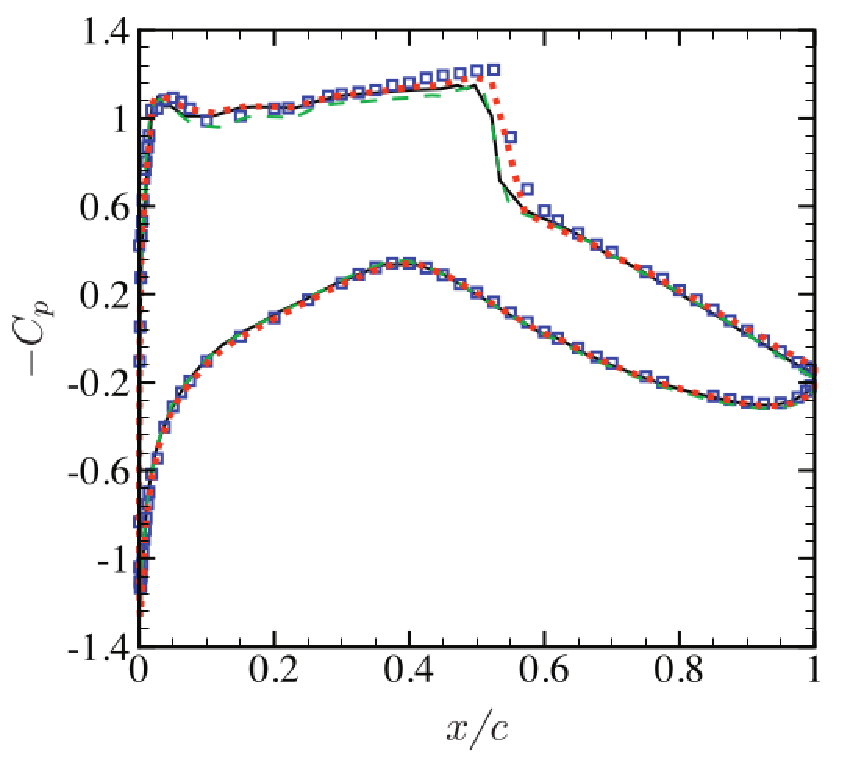
\includegraphics[width=0.5\textwidth]{Cp_RAE2822}
		\caption{RANS del RAE2822: coefficiente di pressione ottenuto da rhoEnergyFoam (linee continue) e da rhoCentralFoam (punti), rispetto a precedenti RANS (linee tratteggiate) e a dati sperimentali (quadrati).}
		\label{Cp_RAE2822}
	\end{figure}
	
	\chapter{Discussion}
	\label{chap:discussion}
	Interpret your findings, compare them to existing literature, and discuss their implications.
	
	\chapter{Conclusion and Future Work}
	\label{chap:conclusion}
	Summarize the research, highlight key findings, and suggest possible future research directions.
	

	%\backmatter
	\cleardoublepage
	\phantomsection % Give this command only if hyperref is loaded
	\addcontentsline{toc}{chapter}{\bibname}
	% Here put the code for the bibliography. You can use BibTeX or
	% the BibLaTeX package or the simple environment thebibliography.
		% References
	\bibliography{references.bib}  % 'references.bib' file 
	%for the bibliography
	%\printbibliography[heading=bibintoc]
	

\end{document}
